\setchapterabstract{本讲回顾了 Transformer 及其 modern variants,重点讨论 normalization (Pre-norm, RMSNorm)、activation functions (ReLU, GeLU, SwiGLU)、position embeddings (absolute, relative, RoPE),并总结 hyperparameter choices、training stability tricks 以及 attention variants (MQA, GQA, sparse attention)。}

\vspace{-10cm}
\chapter{Architectures variations \& Hyperparameters \& Stability tricks}

\vspace{-2cm}

%%%%%%INSERT TOC BELOW 1ST SECTION%%%%%%%%%%%%

{\chaptoc\noindent\begin{minipage}[inner sep=0,outer sep=0]{0.9\linewidth}\section{The Original Transformer \& Modern Variants}\end{minipage}}
\\

\subsection{Review of the Original Transformer}

\begin{figure}[htbp]
  \centering
  \begin{minipage}{0.45\linewidth}
    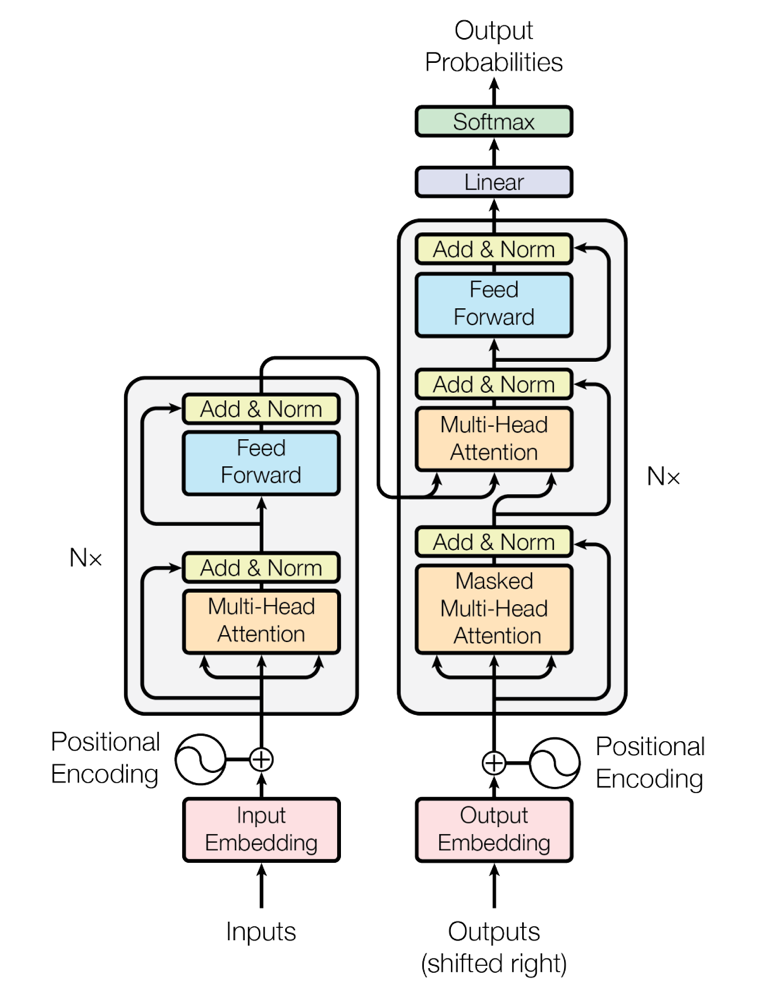
\includegraphics[width=\linewidth]{figs/lec3/lec3.01.png}
    \caption{The original Transformer architecture}
  \end{minipage}
  \hfill
  \begin{minipage}{0.5\linewidth}
    \small
    在Original Transformer Architecture中,我们在选择以下方式来构建Architecture
    \begin{itemize}
    \item \textbf{Norm Type}: Post-norm, LayerNorm
    \item \textbf{FFN Type}: ReLU \\
        \[
        \text{FFN}(z_i) = \text{ReLU}(z_i W_1 + b_1) W_2 + b_2
        \]
    \item \textbf{Position Embedding}: sines and cosines \\
    \begin{align*}
     &\mathrm{PE}(pos,\, 2i)   = \sin \Bigl( pos \,/\, 10000^{\,2i / d_{\mathit{model}}} \Bigr)\\
     &\mathrm{PE}(pos,\, 2i+1) = \cos \Bigl( pos \,/\, 10000^{\,2i / d_{\mathit{model}}} \Bigr)
    \end{align*}

    \end{itemize}

  \end{minipage}
\end{figure}

\MarginImageWithNote
  {figs/lec3/lec3.02.png}
  {\captionof{figure}{Modern Models' Architecture}}
  {}

而这些有许多变体,接下来我们会逐一介绍:
\begin{itemize}
    \item Pre-norm vs. Post-norm
    \item LayerNorm vs. RMSNorm
    \item ReLU, GeLU, *GLU, SwiGLU
    \item Serial vs. Parallel layers
    \item Relative Position Embeddings vs. Absolute Position Embeddings
\end{itemize}

\clearpage
\subsection{Normalization Variants}~{}

\MarginImage
  {figs/lec3/lec3.03.png}
  {\captionof{figure}{Pre-norm vs. Post-norm in residual flow}
  \label{fig:fig3.3}}


\subsubsection{Pre-norm vs. Post-norm in Transformer}~{}

\begin{figure}[htbp]
  \centering
  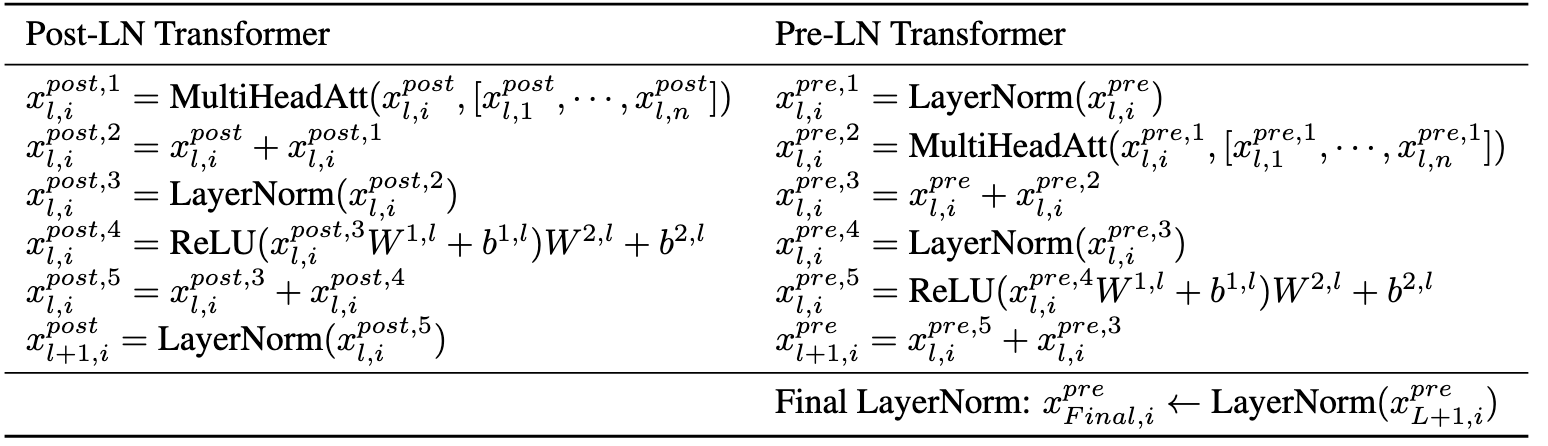
\includegraphics[width=1\linewidth]{figs/lec3/lec3.04.png}
  \captionof{figure}{Post-LN Transformer v.s. Pre-LN Transformer}
  \label{fig:}
\end{figure}

如Figure~\ref{fig:fig3.3}所示,Post-LN 将 LayerNorm 放置在residual signal path 之中,在残差连接之后;而 Pre-LN 将其置于子层输入之前,不置于residual signal path之中。

在论文\textit{On Layer Normalization in the Transformer Architecture}中,作者比较了 Pre-LN 与 Post-LN 的差异,发现 Post-LN 在深层网络中容易出现梯度消失或训练不稳定的问题,
而 Pre-LN 则能够:

\begin{itemize}
  \item Remove warm-up stage
  \item 缓解梯度爆炸与消失问题  
  \item Stability and larger LRs for large networks
\end{itemize}

\paragraph{1. Pre-LayerNorm 可以去除模型对于warm-up阶段的依赖}~{}
\MarginNote{
\Definition{Learning Rate Warm-up Stage}{
Post-LN Transformer 需要先从较小的学习率逐步升高,才能避免训练不稳定
(Popel \& Bojar, 2018)。  

设第 $t$ 次迭代的学习率为 $lr(t)$,训练过程中的最大学习率为 $lr_{\max}$,
给定 warm-up 时间步长 $T_{\text{warm-up}}$,其调度方式为:
\[
lr(t) = \frac{t}{T_{\text{warm-up}}} \, lr_{\max}, \quad t \leq T_{\text{warm-up}}.
\]

在 warm-up 阶段之后,学习率由经典调度器设定,如线性衰减、
逆平方根衰减或特定迭代点的强制衰减(Vaswani et al., 2018)。
}
}

In Figure~\ref{fig:lec3.05}, the x-axis is the epoch number and the y-axis is the BLEU score/validation loss. "w/o warm-up" indicates “without the warm-up stage” while "w/ warm-up" indicates “with the warm-up stage”.\\
In conclusion:
\begin{itemize}
  \item The learning rate warm-up stage is essential for Post-LN Transformer.
  \item The optimization process is sensitive to the value of $T_{\text{warm-up}}$ demanding fine-tuning.
\end{itemize}

这会有两个弊端:
\begin{itemize}
  \item Its configuration significantly affects the final performance. The practitioners need a careful hyper-parameter tuning, which is computationally expensive for large-scale NLP tasks.
  \item The warm-up stage could slow down the optimization. Standard optimization algorithms usually start with a large learning rate for fast convergence. However, when using the warm-up stage, the learning rate has to gradually increase from zero, which may make the training inefficient.
\end{itemize}

  
\MarginImageWithNote
{figs/lec3/lec3.05.png}
{\captionof{figure}{Performance of the models with different learning rate and $T_{\text{warm-up}}$}
  \label{fig:lec3.05}
}

\clearpage
当采取Pre-LayerNorm 后,我们可以安全地去除warm-up阶段的依赖。
\begin{figure}[htbp]
  \centering
  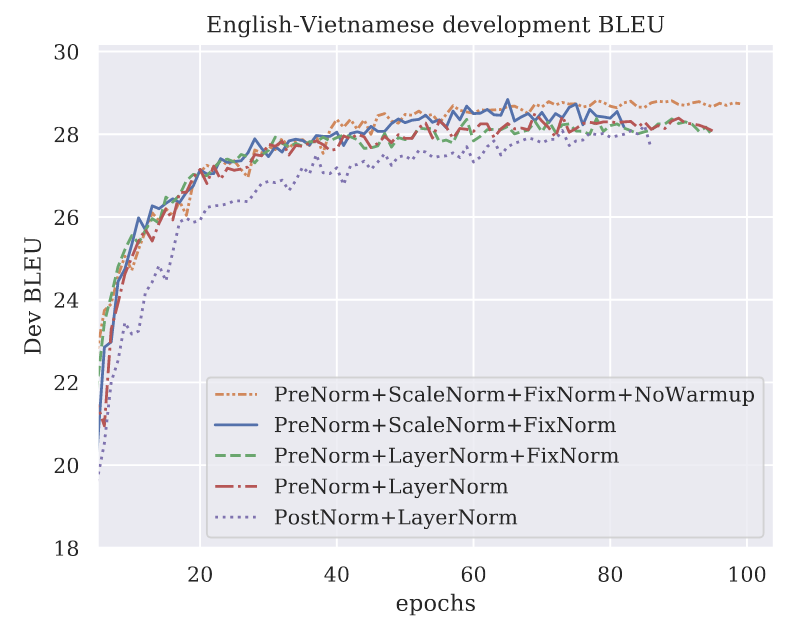
\includegraphics[width=0.8\linewidth]{figs/lec3/lec3.07.png}
  \captionof{figure}{Development BLEU on en→vi with POSTNORM or PRENORM, and with LAYERNORM or SCALENORM.}
\end{figure}

\Proposition{Pre-LayerNorm removes the need for warm-up.}{
Consider a Transformer block with input $\mathbf{x}$, sub-layer function $\mathcal{F}$, and normalization $\text{LN}(\cdot)$.  

\textbf{Post-LN Formulation:}
\[
\mathbf{y} = \text{LN}\big(\mathbf{x} + \mathcal{F}(\mathbf{x})\big).
\]
Backward gradient:
\[
\nabla_{\mathbf{x}} \mathcal{L} = \nabla_{\mathbf{y}}\mathcal{L} \cdot 
\Big( I + J_{\mathcal{F}}(\mathbf{x}) \Big) \cdot J_{\text{LN}}(\mathbf{x}+\mathcal{F}(\mathbf{x})),
\]
where $J$ denotes the Jacobian.  
Since $\text{LN}$ is applied \emph{after} the residual addition, its Jacobian $J_{\text{LN}}$ couples all components, making $\nabla_{\mathbf{x}}$ scale-sensitive.  
A large learning rate can lead to unstable updates $\|\nabla_{\mathbf{x}}\| \gg 1$, hence requiring a warm-up to gradually increase $\eta$.

\textbf{Pre-LN Formulation:}
\[
\mathbf{y} = \mathbf{x} + \mathcal{F}(\text{LN}(\mathbf{x})).
\]
Backward gradient:
\[
\nabla_{\mathbf{x}} \mathcal{L} = \nabla_{\mathbf{y}}\mathcal{L} \cdot 
\Big(I + J_{\mathcal{F}}(\text{LN}(\mathbf{x})) \cdot J_{\text{LN}}(\mathbf{x}) \Big).
\]
Here, normalization is applied \emph{before} the sub-layer.  
Thus the input to $\mathcal{F}$ is always scale-invariant, and the residual path contributes an identity map.  
Therefore the gradient is stabilized around the identity, avoiding exploding/vanishing norms.  

\[
\implies \text{Pre-LN ensures stable optimization, even without warm-up.}
\]
}




\clearpage
\paragraph{2. Pre-LayerNorm 可以缓解梯度爆炸问题}~{}
\\
\begin{figure}[htbp]
  \centering
  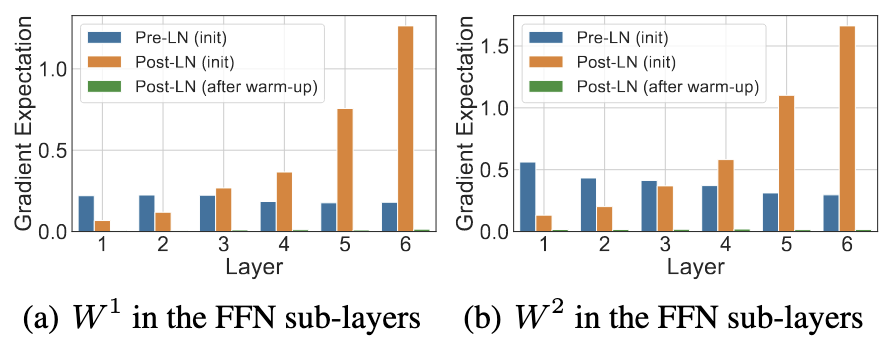
\includegraphics[width=0.65\linewidth]{figs/lec3/lec3.06.png}
  \captionof{figure}{Gradient Attenuation by Pre-LN}
\end{figure}


\begin{figure}[htbp]
  \centering
  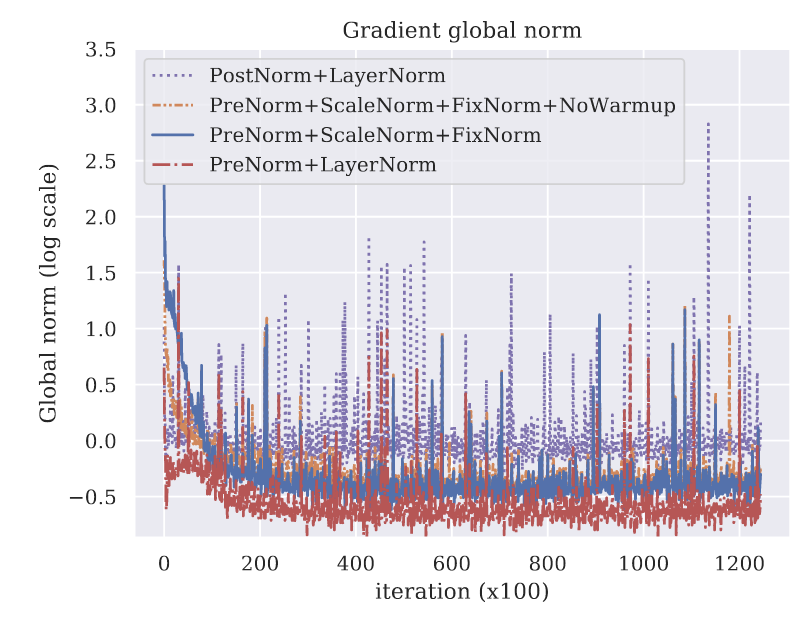
\includegraphics[width=0.65\linewidth]{figs/lec3/lec3.08.png}
  \captionof{figure}{Gradient Spikes}
\end{figure}

\paragraph{3. Pre-LayerNorm 可以提高整体的稳定性并提高Learning Rate加速收敛}~{}
\begin{figure}[htbp]
  \centering
  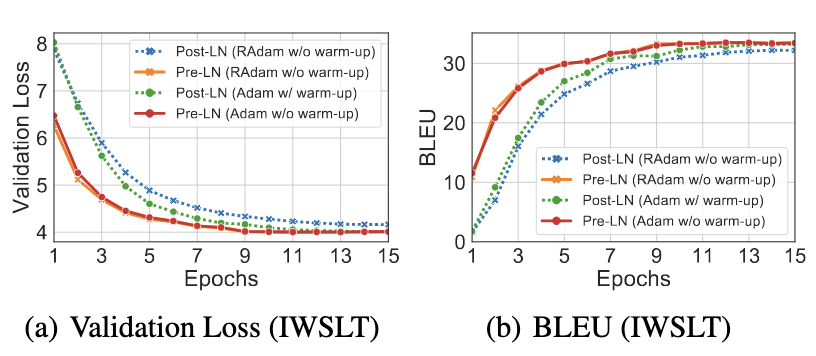
\includegraphics[width=0.65\linewidth]{figs/lec3/lec3.09.png}
  \captionof{figure}{Performances of the models with pre-norm or post-norm}
\end{figure}

\textbf{Almost all modern LMs use pre-norm (but BERT was post-norm)}

\clearpage
\subsubsection{Double Norm}

\begin{figure}[htbp]
  \centering
  \begin{minipage}{0.45\linewidth}
    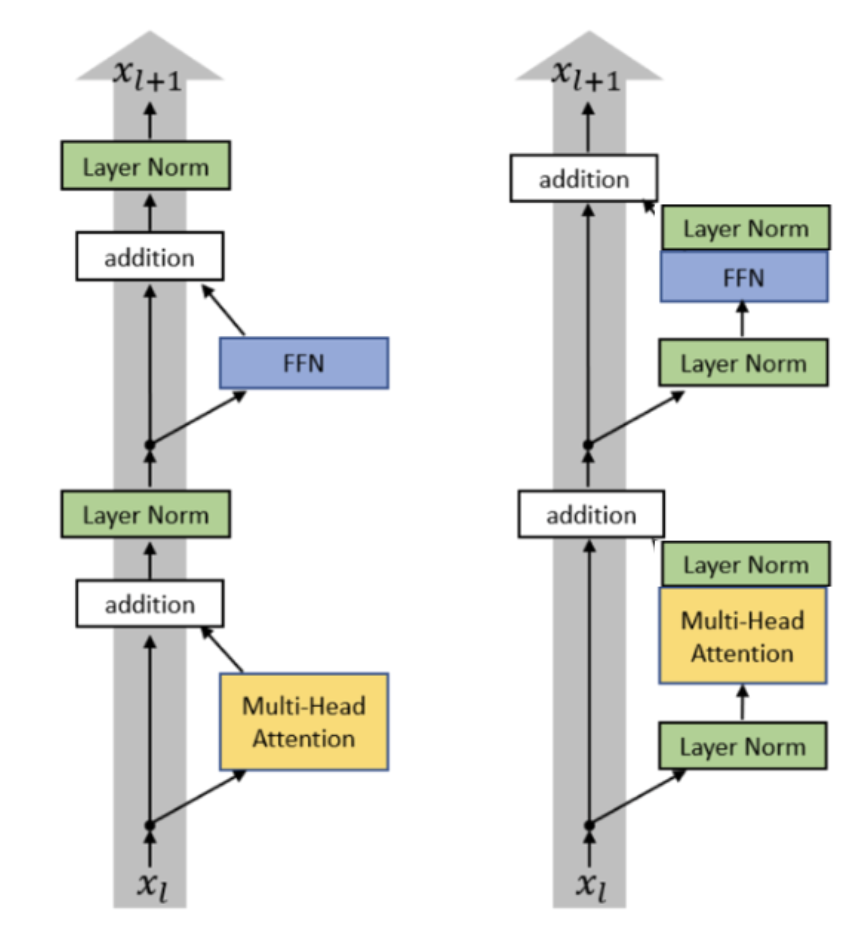
\includegraphics[width=\linewidth]{figs/lec3/lec3.10.png}
    \caption{Transformer with double layernorm }
  \end{minipage}
  \hfill
  \begin{minipage}{0.5\linewidth}
    \small
    \QA
    {Why putting LayerNorms in residual streams is bad?}
    {
    Residual connections provide an identity mapping from lower to higher layers, which is crucial for stable gradient flow in very deep networks.  
    If a LayerNorm is inserted \emph{inside} the residual stream, this identity path is no longer preserved---it is transformed by the normalization operator.  
    As a result, the gradients are no longer guaranteed to propagate cleanly, which can lead to training instability.  
    }
  \end{minipage}
\end{figure}

\textbf{Motivation.}
\begin{itemize}
  \item \emph{Post-LN:} $\mathbf{x}_{l+1} = \text{LN}(\mathbf{x}_l + \mathcal{F}(\mathbf{x}_l))$  
        stabilizes layer-wise distributions but destroys the identity mapping in the residual path, \textbf{leading to unstable gradients and requiring warm-up}.
  \item \emph{Pre-LN:} $\mathbf{x}_{l+1} = \mathbf{x}_l + \mathcal{F}(\text{LN}(\mathbf{x}_l))$  
        preserves the residual identity for stable gradients without warm-up, but lacks normalization after the residual addition, \textbf{causing distribution shift in deep networks}.
\end{itemize}

\textbf{Effect }Double LayerNorm combines the strengths of both: \\ 
\begin{itemize}
  \item \textbf{Norm-in} ($\text{LN}_{\text{in}}$) ensures the input to $\mathcal{F}$ is scale-invariant, preserving stable gradient flow as in Pre-LN.
  \item \textbf{Norm-out} ($\text{LN}_{\text{out}}$) normalizes the residual sum, aligning the output distribution across layers as in Post-LN.
\end{itemize}

Thus, Double LayerNorm avoids the dependency on warm-up while also preventing distribution drift, leading to more stable and scalable training of deep Transformers.

\textbf{Recent Models:} Grok,Gemma 2.



\clearpage
\subsubsection{LayerNorm vs. RMSNorm}

\Definition{Layer Normalization (LayerNorm)}{
给定输入向量 $\mathbf{x} = (x_1, x_2, \dots, x_d) \in \mathbb{R}^d$,LayerNorm 对整个维度做归一化:
\[
\hat{x}_i = \frac{x_i - \mu}{\sqrt{\sigma^2 + \epsilon}}, 
\quad \mu = \frac{1}{d}\sum_{j=1}^d x_j, 
\quad \sigma^2 = \frac{1}{d}\sum_{j=1}^d (x_j - \mu)^2.
\]
最后再进行可学习($\gamma$, $\beta$)的仿射变换:
\[
y_i = \gamma \hat{x}_i + \beta, \quad \gamma, \beta \in \mathbb{R}^d.
\]
它显式地移除了均值并缩放方差,保证归一化后的特征分布具有零均值和单位方差。

\textbf{Notable models:} GPT3/2/1, OPT, GPT-J
}

\Definition{Root Mean Square Normalization (RMSNorm)}{
RMSNorm 省略了均值归一化,仅基于均方根 (RMS) 对输入缩放:
\[
\hat{x}_i = \frac{x_i}{\sqrt{\frac{1}{d}\sum_{j=1}^d x_j^2 + \epsilon}},
\]
再施加可学习的缩放参数($\gamma$):
\[
y_i = \gamma \hat{x}_i, \quad \gamma \in \mathbb{R}^d.
\]
RMSNorm 保持输入方向不变,仅依赖整体幅值的缩放。
\textbf{Notable models:} LLaMA-family, PaLM, Chinchilla
}

\QA{Why RMSNorm?}
{
\begin{itemize}
  \item \textbf{Fewer operations} No mean calculation
  \item \textbf{Fewer parameters} No bias term to store
\end{itemize}
}


\MarginImageWithNote
{figs/lec3/lec3.11.png}
{\captionof{figure}{Proportion of FLOPs across different operations}}
{\textbf{Matrix multipliers are the \textit{vast majority of FLOPs (and memory)}}}

\MarginImageWithNote
{figs/lec3/lec3.12.png}
{\captionof{figure}{Proportion of Runtime across different operations}}
{\textbf{RMSNorm can still matter due to the importance \textit{data movement.}}}

\Remark{
\textbf{  FLOPS are not runtime!
}}

\MarginImageWithNote
{figs/lec3/lec3.13.png}
{\captionof{figure}{FLOPS and FLOP-to-memory ratio in Transformer}}

\begin{figure}[htbp]
  \centering
  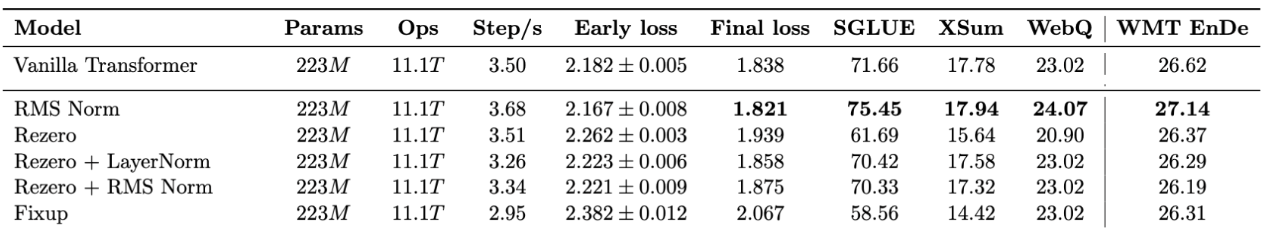
\includegraphics[width=0.8\linewidth]{figs/lec3/lec3.14.png}
  \captionof{figure}{RMSNorm runtime}
\end{figure}

\Insight{Dropping Bias Terms}{
Most modern Transformers omit explicit bias terms.  

\textbf{Original Transformer (Vaswani et al., 2017):}
\[
\text{FFN}(x) = \max\!\bigl(0,\, xW_1 + b_1\bigr)W_2 + b_2
\]

\textbf{Typical Modern Implementation (non-gated):}
\[
\text{FFN}(x) = \sigma(xW_1)W_2
\]

\textbf{Reasons:}  
{\color{dblue}{
- \emph{Memory efficiency:} Similar to RMSNorm, removing biases reduces parameter count and memory footprint.  \\
- \emph{Optimization stability:} Empirically, biases contribute little to training stability in deep architectures, so omitting them avoids redundant parameters.  
}}
}

\clearpage
\subsection{Activation Variants}
\paragraph{A few of the common activations}~{}

\MarginImageWithNote
  {figs/lec3/lec3.15.png}
  {\captionof{figure}{ReLU vs. GELU}}
  {ReLU is flat  for $x<0$, while GELU provides a smoother transition with a small bump around the origin.}

% ---------- 非门控 FFN:与论文一致的无偏置写法 ----------
\begin{itemize}
  \item \textbf{ReLU (Rectified Linear Unit):}
  \begin{align*}
    \mathrm{ReLU}(z) &= \max(0, z), \\
    \mathrm{FFN}_{\mathrm{ReLU}}(x, W_1, W_2, b_1, b_2) 
      &= \max(0,\, xW_1+b_1)\,W_2 + b_2.
    \tag{3.1}
  \end{align*}

  \item \textbf{GELU (Gaussian Error Linear Unit):}
  \begin{align*}
    \mathrm{GELU}(z) &= z \cdot \Phi(z) \\
                     &= \frac{z}{2}\Bigl(1+\mathrm{erf}\!\left(\tfrac{z}{\sqrt{2}}\right)\Bigr), \\
    \mathrm{FFN}_{\mathrm{GELU}}(x, W_1, W_2, b_1, b_2) 
      &= \mathrm{GELU}(xW_1+b_1)\,W_2 + b_2.
    \tag{3.2}
  \end{align*}
  其中
  \[
  \Phi(z)=\tfrac{1}{2}\Bigl(1+\mathrm{erf}\!\left(\tfrac{z}{\sqrt{2}}\right)\Bigr),
  \quad
  \mathrm{erf}(u)=\tfrac{2}{\sqrt{\pi}}\int_0^u e^{-t^2}\,dt.
  \]
\end{itemize}


\paragraph{Gated activations(*GLU)}~{}

\MarginNote{
\textbf{Gated FFN 参数量解释:}\\[0.3em]
普通 FFN: 
$d_{\mathrm{model}} \!\to\! d_{\mathrm{ff}} \!\to\! d_{\mathrm{model}}$。\\
Gated FFN: 
需要两条分支,若仍用原始 $d_{\mathrm{ff}}$,参数量几乎翻倍。\\[0.3em]
解决方法:把每条分支的维度设为原来的 $\tfrac{2}{3}d_{\mathrm{ff}}$。这样两条分支加起来的参数量 $\approx$ 原始 FFN,但通过门控乘法获得更强表达能力。
}

GLU-style activations replace this with a gated version:
\[
  {\color{tred}{\max(0,\,xW_1)}} 
  \;\;\longrightarrow\;\;
  {\color{dblue}{\max(0,\,xW_1)}} \odot (xV),
\]
where $(xV)$ is the gate vector applied entrywise.

\Definition{Entrywise (Hadamard) Product $\odot$}{
Given two vectors $\mathbf{a}, \mathbf{b} \in \mathbb{R}^d$, their entrywise (Hadamard, element-wise) product is
\[
(\mathbf{a} \odot \mathbf{b})_i = a_i \, b_i, \quad i=1,\dots,d.
\]
In gated feed-forward networks (GLU and its variants), one branch generates the main signal while the other generates a gate vector; the Hadamard product $\odot$ applies the gate to each dimension individually.
}

\MarginImageWithNote
{figs/lec3/lec3.16.png}
{\captionof{figure}{GLUE Language-Understanding Benchmark}}
{
\textbf{Swish$_1$ vs. Swish$_\beta$}\\[0.3em]
一般形式:$\mathrm{Swish}_\beta(x)=x\sigma(\beta x)$.\\
- $\beta=1$ 固定时 $\Rightarrow$ Swish$_1$.\\
- $\beta$ 可调时 $\Rightarrow$ Swish$_\beta$, 曲线形状可随 $\beta$ 改变:$\beta\to0$ 近似线性,$\beta\to\infty$ 接近 ReLU.
}

\begin{itemize}
  \item \textbf{ReGLU (ReLU Gated Linear Unit):}
  \begin{align*}
    \mathrm{ReGLU}(x) &= \max(0,\, xW_1) \odot (xV), \\
    \mathrm{FFN}(x)   &= \mathrm{ReGLU}(x)W_2.
  \end{align*}
  其中第一项是 ReLU 激活后的主分支,第二项 $(xV)$ 作为门控向量,两者做 Hadamard product。

  \item \textbf{GeGLU (GELU Gated Linear Unit):}
  \begin{align*}
    \mathrm{GeGLU}(x) &= \mathrm{GELU}(xW_1) \odot (xV), \\
    \mathrm{FFN}(x)   &= \mathrm{GeGLU}(x)W_2.
  \end{align*}
  将 ReLU 换成 GELU,使得门控更平滑,广泛用于 GPT-3、PaLM 等大模型。

  \item \textbf{SwiGLU (Swish Gated Linear Unit):}
  \begin{align*}
    \mathrm{SwiGLU}(x) &= \mathrm{Swish_1}(xW_1) \odot (xV), \\
    \mathrm{FFN}(x)    &= \mathrm{SwiGLU}(x)W_2,
  \end{align*}
\end{itemize}




\clearpage
\subsection{Serial vs. Parallel layers}

\MarginNote{
\QA{Why faster?}{
In parallel blocks, both Attention and MLP take the same $\mathrm{LN}(x)$ as input. \\
$\Rightarrow$ Their input projections can be \textit{fused} into a single large matmul: 
\[
[xW_Q,\, xW_K,\, xW_V,\, xW_1] = x \cdot W
\] 
instead of separate ones.\\
This reduces GPU kernel launches \& memory traffic, yielding about \textbf{15\% speedup} at large scale.
} 
\textbf{Recent Models:} Cohere Command A, Falcon 2 11B, Command R+
}


\begin{figure}[htbp]
  \centering
  \begin{minipage}{0.45\linewidth}
    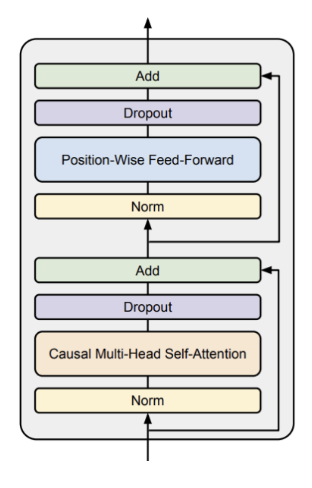
\includegraphics[width=\linewidth]{figs/lec3/lec3.17.png}
    \caption{A transformer block in original transformer}
  \end{minipage}
  \hfill
  \begin{minipage}{0.5\linewidth}
    \small
      Normal Transformer blocks are \textit{serial}: they compute attention, then the MLP. \\
      Now a few models (e.g., GPT-J, PaLM, GPT-NeoX) adopt \textit{parallel layers}. \\
      \textbf{Serial formulation (standard):}  \\
      \[
        y = x + \mathrm{MLP}\bigl(\mathrm{LN}(x + \mathrm{Attention}(\mathrm{LN}(x)))\bigr)
      \]
      \textbf{Parallel formulation:}
      \[
        y = x + \mathrm{MLP}(\mathrm{LN}(x)) + \mathrm{Attention}(\mathrm{LN}(x))
      \]

      Parallel formulation allows the MLP and Attention input projections to be computed together, giving about 
      \textbf{15\% faster training at large scale}. \\ 
      Empirically, PaLM observed \textit{no quality degradation at 62B scale}, so the effect is considered quality-neutral at 540B.
  \end{minipage}
\end{figure}


\clearpage
\subsection{RoPE: Rotary Position Embeddings}

\paragraph{A few of commom embeddings}~{}
\\
\MarginNote{
Recall: For a token $x$ at position $i$: 
\[
\mathrm{Embed}(x,i) = v_x + \mathrm{PE}_i
\]
}

\begin{itemize}
  \item \textbf{Sine embeddings:} add sines and cosines that enable localization
  \begin{align*}
    \mathrm{PE}_{(pos,2i)}   &= \sin\!\left(\frac{pos}{10000^{2i/d_{\text{model}}}}\right), \\
    \mathrm{PE}_{(pos,2i+1)} &= \cos\!\left(\frac{pos}{10000^{2i/d_{\text{model}}}}\right),
  \end{align*}
  where $pos$ is the position index, $i$ is the dimension index.

\item \textbf{Absolute embeddings:} add a position vector to the embedding
  \begin{align*}
    \mathrm{Embed}(x,i) &= v_x + u_i
  \end{align*}
  where 
  \begin{itemize}
    \item $v_x \in \mathbb{R}^{d_z}$ : token $x$ 的词向量 (word embedding),
    \item $u_i \in \mathbb{R}^{d_z}$ : 位置 $i$ 的绝对位置向量 (absolute positional embedding)。
  \end{itemize}

  \item \textbf{Relative embeddings:} add a bias term to the \textit{attention computation}
  \begin{align*}
    e_{ij} &= \frac{x_i W^Q \,(x_j W^K + {\color{tred}a_{ij}^K)}^T}{\sqrt{d_z}}
  \end{align*}
  where
  \begin{itemize}
    \item $x_i \in \mathbb{R}^{d_z}$ : 第 $i$ 个位置的输入表示,
    \item $W^Q, W^K \in \mathbb{R}^{d_z \times d_z}$ : query 与 key 的投影矩阵,
    \item $x_i W^Q$ : 位置 $i$ 的 query 向量,
    \item $x_j W^K$ : 位置 $j$ 的 key 向量,
    \item {\color{tred}$a_{ij}^K$} $\in  \mathbb{R}^{d_z}$ : 与相对距离 $(i-j)$ 相关的相对位置嵌入,
    \item 分母 $\sqrt{d_z}$ : 标准 attention 中的缩放因子。
  \end{itemize}
  Thus, $e_{ij}$ is the attention score between position $i$ and $j$, augmented with relative positional information.
\end{itemize}

\paragraph{High level thought process: Relativity }~{}
\\
\Remark{
A \textbf{relative position embedding} should be a mapping $f(x,i)$ such that
\[
\langle f(x,i), f(y,j) \rangle \;=\; g(x,y,\, i-j).
\]
That is, the attention score depends not only on the content $(x,y)$, 
but also only on the \textit{relative position} $(i-j)$, rather than the absolute indices $i$ or $j$.
}

How do existing embeddings not fulfill this goal?

\begin{itemize}
  \item \textbf{Sine:} Has various cross-terms that are not purely relative. 
  \[
    \langle \mathrm{Embed}(x,i), \mathrm{Embed}(y,j) \rangle 
      = \langle v_x, v_y \rangle 
      + \langle \mathrm{PE}_i, v_y \rangle + \cdots
  \]
  So the score depends on both token embeddings and absolute position terms.

  \item \textbf{Absolute:} Obviously not relative --- embeddings $u_i$ are tied to absolute positions $i$ rather than $(i-j)$.

  \item \textbf{Relative embeddings:} 
  \[
    e_{ij} = \frac{x_i W^Q (x_j W^K + a_{ij}^K)^T}{\sqrt{d_z}}
  \]
  encodes relative information, but this modification is no longer a \textbf{pure inner product} between query and key; it adds an extra bias term. 
\end{itemize}

\paragraph{RoPE: rotary position embeddings}~{}
\QA{How can we solve this problem?}
{
\begin{itemize}
  \item Our embeddings should be invariant to absolute positions.
  \item The inner products are invariante to arbitrary rotations.
\end{itemize}
}

\subsubsection*{A 2D case}

\MarginNote{
  \Definition{Euler's Formula}{
    在复数平面上,$e^{i\theta} = \cos\theta + i\sin\theta$。
    乘上 $e^{i\theta}$ 相当于把二维向量旋转角度 $\theta$:
    \begin{align*}
      (a+ib)\,e^{i\theta}
      &= (a\cos\theta - b\sin\theta) \\
      &+ i(a\sin\theta + b\cos\theta).
    \end{align*}
    因此,复数乘以 $e^{i\theta}$ 本质上就是一个二维旋转。
  }
}   


在二维情况下,我们可以把词向量 $\mathbf{x}_m$ 经过线性变换 $\mathbf{W}_q$ 或 $\mathbf{W}_k$ 后,
再乘上一个旋转因子 $e^{i m \theta}$ 或 $e^{i n \theta}$,分别得到

\begin{align*}
f_q(\mathbf{x}_m,m) &= (\mathbf{W}_q \mathbf{x}_m) e^{i m \theta},\\
f_k(\mathbf{x}_n,n) &= (\mathbf{W}_k \mathbf{x}_n) e^{i n \theta}.\\
g(\mathbf{x}_m,\mathbf{x}_n,m-n) 
&= \operatorname{Re}\!\left[(\mathbf{W}_q \mathbf{x}_m)(\mathbf{W}_k \mathbf{x}_n)^{*} e^{i (m-n)\theta}\right],
\end{align*}

其中 $(\cdot)^*$ 表示共轭复数,$\operatorname{Re}[\cdot]$ 取实部。
这个形式表明:打分结果只依赖位置差 $(m-n)$,从而实现了相对位置编码。

进一步地,$f_q$ 也可以写成矩阵形式:
\begin{align*}
f_{q}(\mathbf{x}_m, m) &=
\begin{pmatrix}
\cos(m\theta) & -\sin(m\theta) \\
\sin(m\theta) &  \cos(m\theta)
\end{pmatrix}
\begin{pmatrix}
W^{(11)}_q & W^{(12)}_q \\
W^{(21)}_q & W^{(22)}_q
\end{pmatrix}
\begin{pmatrix}
x^{(1)}_m \\
x^{(2)}_m
\end{pmatrix}.\\
&=
\begin{pmatrix}
\cos(m\theta) & -\sin(m\theta) \\
\sin(m\theta) &  \cos(m\theta)
\end{pmatrix}
\begin{pmatrix}
q^{(1)}_m \\
q^{(2)}_m
\end{pmatrix}
\end{align*}
看到这里会发现,这不就是 query 向量乘以了一个旋转矩阵吗?这就是为什么叫做旋转位置编码的原因。



同理,$f_k$ 也可以写成矩阵形式:
\begin{align*}
f_{k}(\mathbf{x}_n, n) &=
\begin{pmatrix}
\cos(n\theta) & -\sin(n\theta) \\
\sin(n\theta) &  \cos(n\theta)
\end{pmatrix}
\begin{pmatrix}
W^{(11)}_k & W^{(12)}_k \\
W^{(21)}_k & W^{(22)}_k
\end{pmatrix}
\begin{pmatrix}
x^{(1)}_n \\
x^{(2)}_n
\end{pmatrix}.\\
&=
\begin{pmatrix}
\cos(n\theta) & -\sin(n\theta) \\
\sin(n\theta) &  \cos(n\theta)
\end{pmatrix}
\begin{pmatrix}
k^{(1)}_n \\
k^{(2)}_n
\end{pmatrix}
\end{align*}

这里的 $f_q,f_k$ 可以统一表示为:
\[
f_{\{q, k\}}(\mathbf{x}_m, m) =
\begin{pmatrix}
\cos(m\theta) & -\sin(m\theta) \\
\sin(m\theta) &  \cos(m\theta)
\end{pmatrix}
\begin{pmatrix}
W^{(11)}_{\{q, k\}} & W^{(12)}_{\{q, k\}} \\
W^{(21)}_{\{q, k\}} & W^{(22)}_{\{q, k\}}
\end{pmatrix}
\begin{pmatrix}
x^{(1)}_m \\
x^{(2)}_m
\end{pmatrix}.
\]


最终 $g(\mathbf{x}_m,\mathbf{x}_n,m-n)$ 可以表示如下:
\begin{equation*}
g(\mathbf{x}_m,\mathbf{x}_n,m-n) =
\begin{pmatrix}
q^{(1)}_m & q^{(2)}_m
\end{pmatrix}
\begin{pmatrix}
\cos((m-n)\theta) & -\sin((m-n)\theta) \\
\sin((m-n)\theta) &  \cos((m-n)\theta)
\end{pmatrix}
\begin{pmatrix}
k^{(1)}_n \\
k^{(2)}_n
\end{pmatrix}.
\end{equation*}





直观理解:RoPE 的做法就是“先线性变换,再按照位置索引旋转一个角度”,
这样点积相似度天然包含了相对位置信息。

\begin{figure}[htbp]
  \centering
  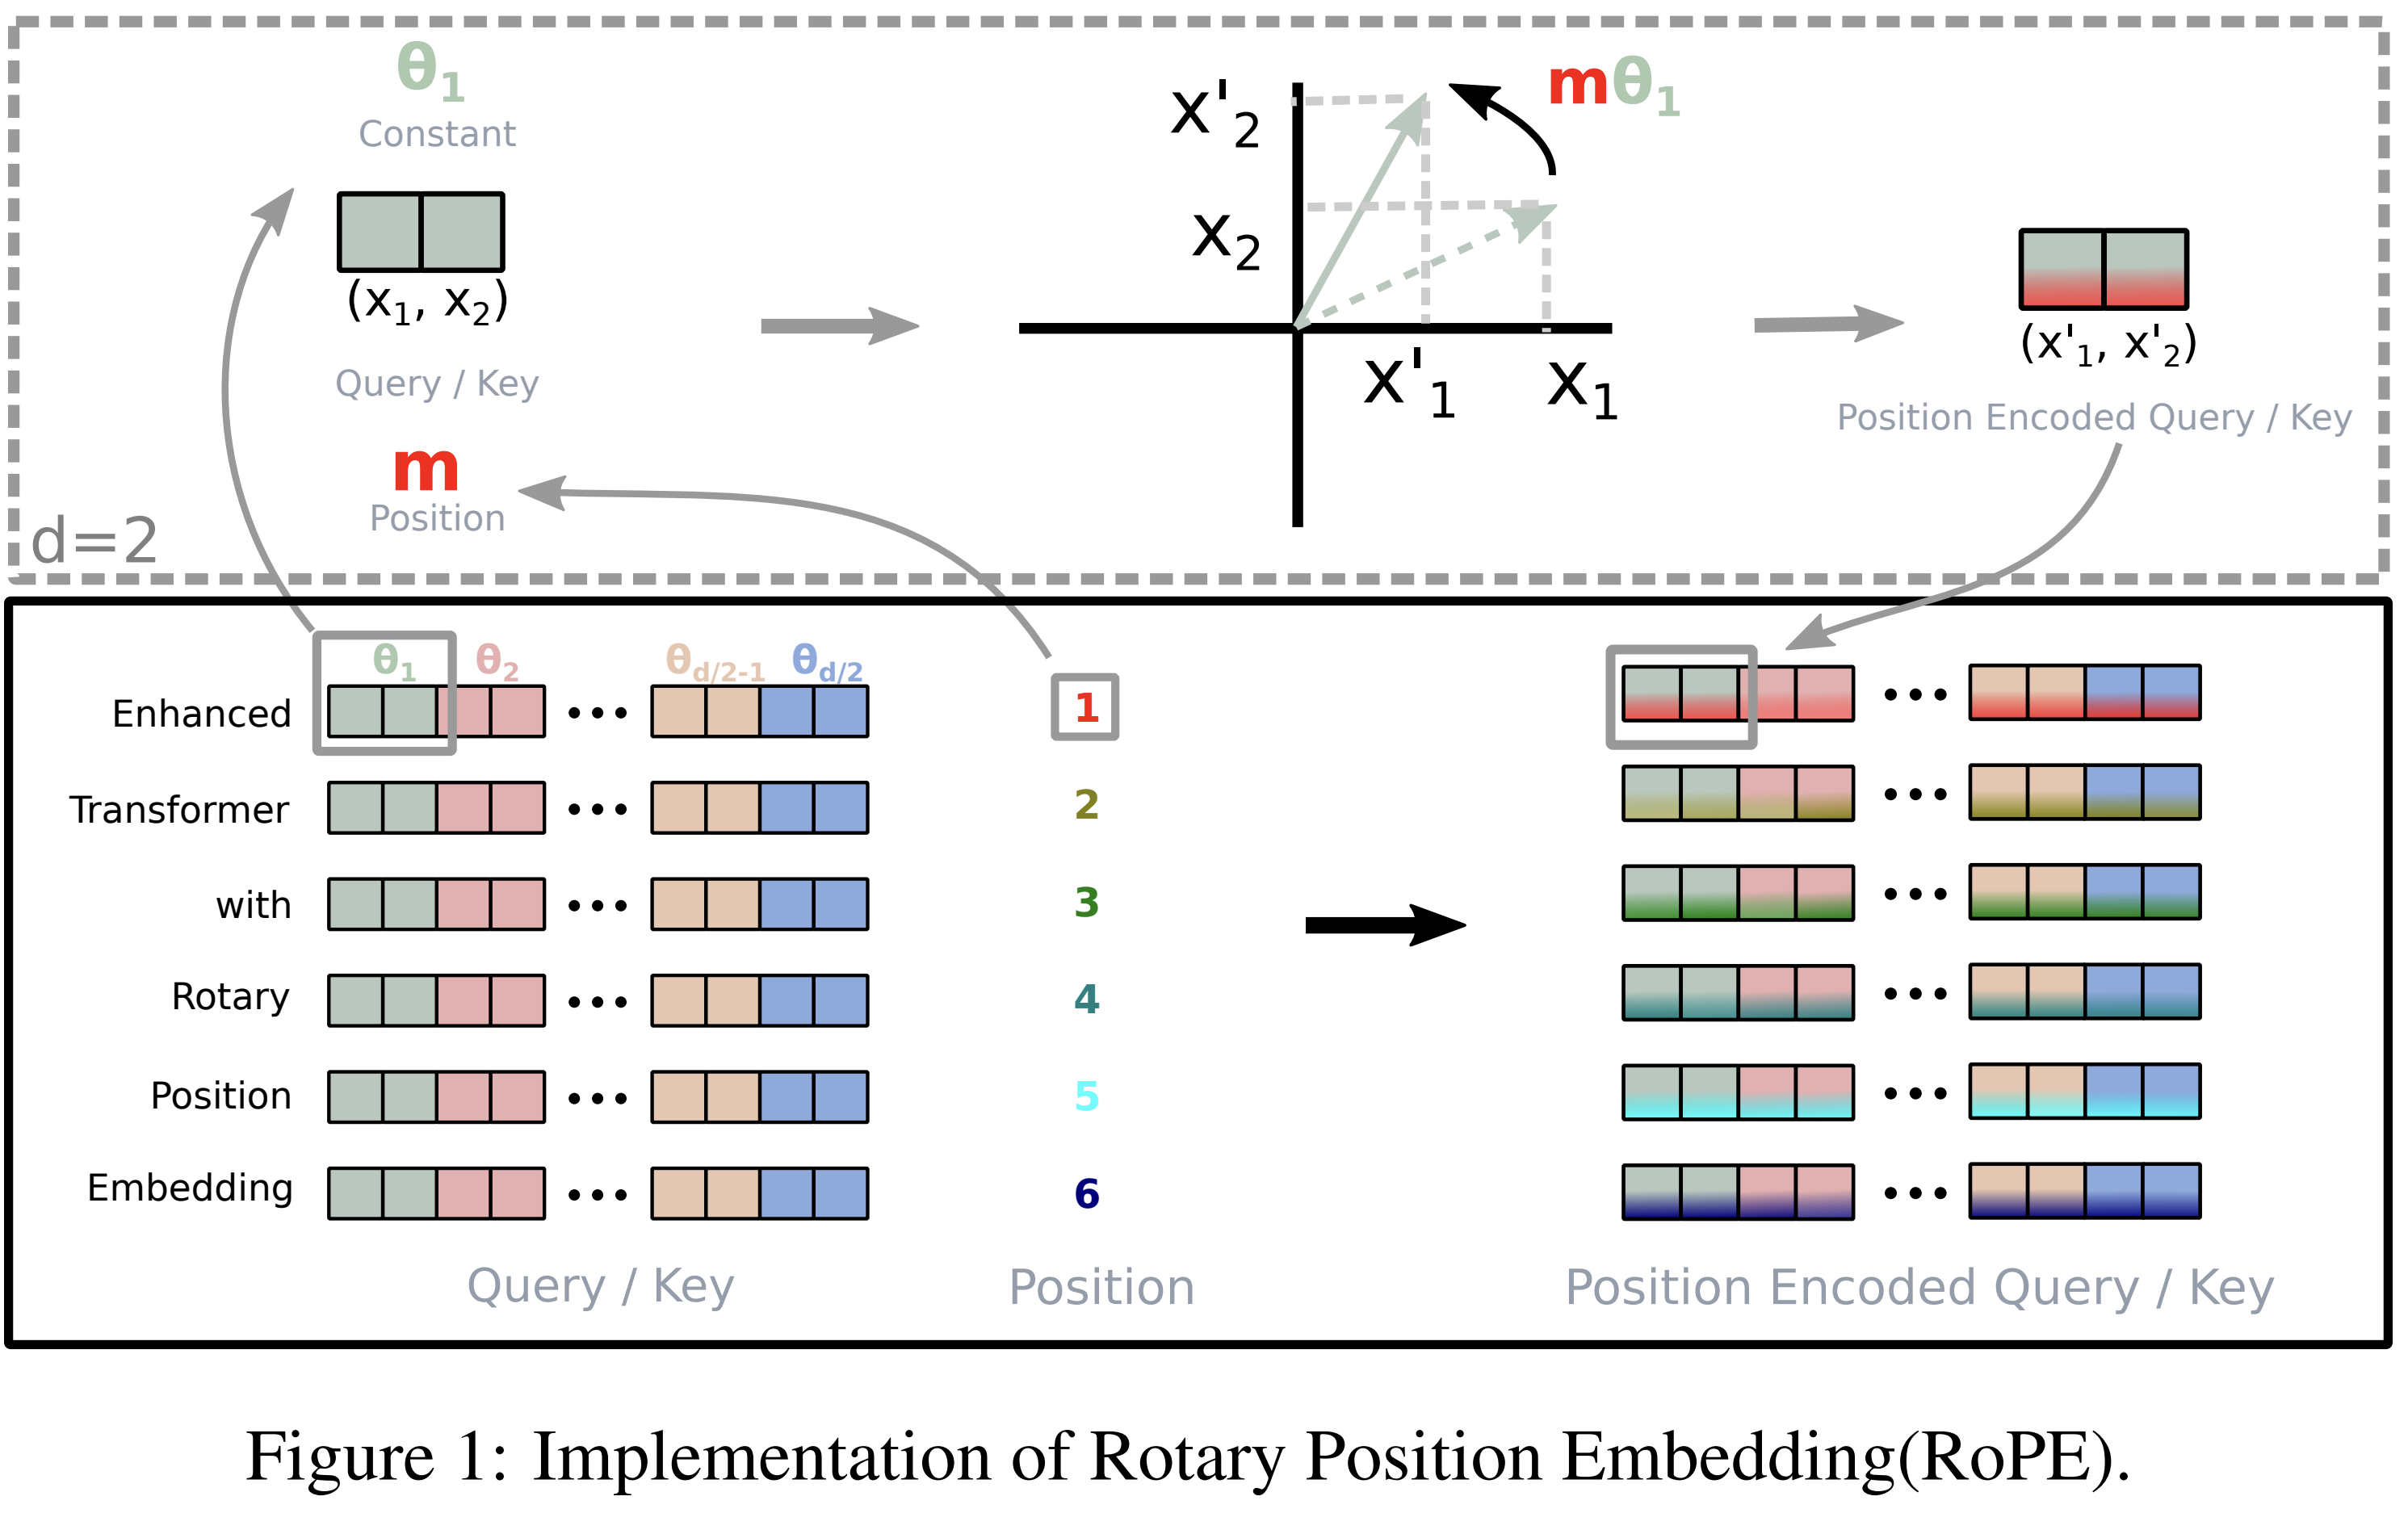
\includegraphics[width=0.8\linewidth]{figs/lec3/lec3.18.png}
  \captionof{figure}{Implementation of Rotary Position Embedding(RoPE).}
\end{figure}


\subsubsection{General form}~{}

从二维情况出发,我们希望推广到任意偶数维度 $d$。设 $\mathbf{x}_i \in \mathbb{R}^d$,我们将 $d$ 维空间划分为 $d/2$ 个二维子空间,并在每个子空间内独立应用二维旋转。利用内积的线性性,可以将 $f_{\{q, k\}}$ 统一写作:
\begin{equation*}
	f_{\{q, k\}}(\mathbf{x}_m, m) 
	= \mathbf{R}^d_{\Theta, m}\,\mathbf{W}_{\{q, k\}}\,\mathbf{x}_m,
	\label{fn:rope-fqk}
\end{equation*}
其中 $\mathbf{R}^d_{\Theta,m}$ 是 $d\times d$ 的分块对角旋转矩阵:
\begin{equation*}    
	\mathbf{R}^d_{\Theta,m} = 
	\begin{pmatrix}
		\cos(m\theta_1)& -\sin(m\theta_1)&0&0&\cdots&0&0\\
		\sin(m\theta_1)& \cos(m\theta_1)&0&0&\cdots&0&0 \\
		0&0&\cos(m\theta_2)& -\sin(m\theta_2)&\cdots&0&0\\
		0&0&\sin(m\theta_2)& \cos(m\theta_2)&\cdots&0&0 \\
		\vdots&\vdots&\vdots&\vdots&\ddots&\vdots&\vdots\\
		0&0&0&0&\cdots&\cos(m\theta_{d/2})& -\sin(m\theta_{d/2})\\
		0&0&0&0&\cdots&\sin(m\theta_{d/2})& \cos(m\theta_{d/2})
	\end{pmatrix},
	\label{fn:rope-RMat}
\end{equation*}

其中参数集合为
\[
\Theta = \Bigl\{\,\theta_i = 10000^{-\tfrac{2(i-1)}{d}},\; i=1,2,\dots,d/2\Bigr\}.
\]

这种结构本质上就是在每个二维子空间内进行旋转,并通过分块对角的拼接推广到 $d$ 维。

\vspace{0.5em}
将 RoPE 应用于自注意力机制,有:
\begin{equation}
	\mathbf{q}_m^{\top}\mathbf{k}_n
	= \bigl(\mathbf{R}^d_{\Theta, m}\mathbf{W}_q\mathbf{x}_m\bigr)^{\!\top}
	\bigl(\mathbf{R}^d_{\Theta, n}\mathbf{W}_k\mathbf{x}_n\bigr)
	= \mathbf{x}_m^{\top}\mathbf{W}_q^\top \mathbf{R}^d_{\Theta, n-m}\mathbf{W}_k\mathbf{x}_n,
	\label{fn:rope-qk}
\end{equation}
其中
\[
\mathbf{R}^d_{\Theta, n-m} = (\mathbf{R}^d_{\Theta, m})^\top \mathbf{R}^d_{\Theta, n}.
\]

需要注意的是,$\mathbf{R}^d_{\Theta,m}$ 是正交矩阵,保证了在引入位置编码时不会破坏数值稳定性。另外,由于 $\mathbf{R}^d_{\Theta}$ 的稀疏分块结构,直接进行矩阵乘法并不高效;在实际实现中通常采用对偶维度成对旋转的写法来避免显式构造整个矩阵。

\subsection{Properties of RoPE}
\label{sec:prop-of-RoPE}

\paragraph{长程衰减 (Long-term decay).} 
在 RoPE 的设计中,我们为每一对维度分配一个频率参数 $\theta_i=10000^{-2i/d}$。  
这样的设置带来一个重要性质:当两个 token 的相对位置差 $(m-n)$ 逐渐增大时,它们的旋转角度差也会逐渐增大,从而使得内积的结果逐渐减小。  
这意味着,随着相对距离变大,query 和 key 之间的相似度会自动衰减,体现了“距离越远,关联越弱”的直觉。  
这一性质保证了 RoPE 在编码长文本时能够自然地控制长程依赖的强度。

\paragraph{结合线性注意力 (RoPE with linear attention).} 
我们知道自注意力机制可以写成一个通用的加权平均形式:
\begin{equation}
	\operatorname{Attention}(\mathbf{Q},\mathbf{K},\mathbf{V})_m
	= \frac{\sum_{n=1}^{N}\operatorname{sim}(\mathbf{q}_m,\mathbf{k}_n)\,\mathbf{v}_n}
	{\sum_{n=1}^{N}\operatorname{sim}(\mathbf{q}_m,\mathbf{k}_n)}.
	\label{fn:atten-full}
\end{equation}

原始的自注意力选择 $\operatorname{sim}(\mathbf{q}_m,\mathbf{k}_n)=\exp(\mathbf{q}_m^\top \mathbf{k}_n / \sqrt{d})$,需要对每一对 $(m,n)$ 计算内积,复杂度是 $\mathcal{O}(N^2)$。  
为了降低计算复杂度,线性注意力提出把相似度函数改写为可分解的形式:

\begin{equation}
	\operatorname{Attention}(\mathbf{Q},\mathbf{K},\mathbf{V})_m
	= \frac{\sum_{n=1}^{N}\phi(\mathbf{q}_m)^\top \varphi(\mathbf{k}_n)\,\mathbf{v}_n}
	{\sum_{n=1}^{N}\phi(\mathbf{q}_m)^\top \varphi(\mathbf{k}_n)},
	\label{fn:linear-attention}
\end{equation}
其中 $\phi(\cdot),\varphi(\cdot)$ 是一些非负函数(例如可以取 $\operatorname{elu}(x)+1$ 或者 softmax)。  
这种改写利用了矩阵乘法的结合律,可以先把 $\varphi(\mathbf{k}_n)\mathbf{v}_n$ 累加,再和 $\phi(\mathbf{q}_m)$ 相乘,从而避免显式计算所有 $\mathcal{O}(N^2)$ 的内积。

\medskip
那么 RoPE 如何与线性注意力结合呢?  
关键在于:RoPE 通过旋转矩阵 $\mathbf{R}^d_{\Theta,m}$ 注入位置信息,而旋转矩阵是正交的,不会改变向量的模长。  
因此我们可以在 $\phi(\mathbf{q}_m)$ 和 $\varphi(\mathbf{k}_n)$ 的输出之后,再乘上旋转矩阵,即:
\begin{equation}
	\operatorname{Attention}(\mathbf{Q},\mathbf{K},\mathbf{V})_m
	= \frac{\sum_{n=1}^{N}\big(\mathbf{R}^d_{\Theta,m}\phi(\mathbf{q}_m)\big)^\top
	\big(\mathbf{R}^d_{\Theta,n}\varphi(\mathbf{k}_n)\big)\,\mathbf{v}_n}
	{\sum_{n=1}^{N}\phi(\mathbf{q}_m)^\top \varphi(\mathbf{k}_n)}.
	\label{fn:linear-rope}
\end{equation}

\paragraph{说明.} 
在这里,分母保持不变,以避免出现除以零的风险。分子部分由于旋转可能引入负值,因此得到的注意力权重并不一定是严格的概率分布。  
但这种形式仍然能正确工作,并且成功地将相对位置信息注入到线性注意力中。

\MarginImageWithNote
{figs/lec3/lec3.19.png}
{\captionof{figure}{Implementation and code for RoPE}}
{\textbf{NOTE:} embedding at \textit{each attention operation} to enforce positive invariance.}


\clearpage
{\chaptoc\noindent\begin{minipage}[inner sep=0,outer sep=0]{0.9\linewidth}\section{Hyperparameters}\end{minipage}}
\\

\subsection{Feedforward Dimension Ratio}

There are two dimensions that are relevant -- the Feedforward dimension $(d_{\mathrm{ff}})$ and the model dimension $(d_{\mathrm{model}})$.
    
\begin{equation}
\mathrm{FFN}_{\mathrm{ReLU}}(x, W_1, W_2, b_1, b_2) 
= \max(0,\, xW_1+b_1)\,W_2 + b_2,
\end{equation}
其中各个部分与 $d_{\mathrm{model}}$ 和 $d_{\mathrm{ff}}$ 的关系如下:

\begin{itemize}
  \item 输入向量 $x \in \mathbb{R}^{d_{\mathrm{model}}}$。
  \item $W_1 \in \mathbb{R}^{d_{\mathrm{model}} \times d_{\mathrm{ff}}}$:把维度从 $d_{\mathrm{model}}$ 投影到 $d_{\mathrm{ff}}$。
  \item $b_1 \in \mathbb{R}^{d_{\mathrm{ff}}}$:对应的偏置。
  \item $\max(0,\cdot)$:ReLU 激活,$\mathbb{R}^{d_{\mathrm{model}}}$ $\rightarrow$ $\mathbb{R}^d_{\mathrm{ff}}$。
  \item $W_2 \in \mathbb{R}^{d_{\mathrm{ff}} \times d_{\mathrm{model}}}$:把维度从 $d_{\mathrm{ff}}$ 投影回 $d_{\mathrm{model}}$。
  \item $b_2 \in \mathbb{R}^{d_{\mathrm{model}}}$:对应的偏置。
  \item 最终输出 $\in \mathbb{R}^{d_{\mathrm{model}}}$,与输入维度相同,方便残差连接。
\end{itemize}

因此,$d_{\mathrm{model}}$ 决定了模型表示的基本维度,而 $d_{\mathrm{ff}}$ 决定了前馈层的中间容量.
通常来说:

\textbf{\[
d_{\mathrm{ff}} = 4 d_{\mathrm{model}}
\]}

但也有一些例外:
\subsubsection{Exception 1 - GLU variants}~{}

在GLU这一部分,我们有提到过,为了保证整体的参数量与Not Gated FFN一致,所以$d_{\mathrm{ff-GLU}} = \frac{2}{3} d_{\mathrm{ff}}$

\begin{figure}[htbp]
  \centering
  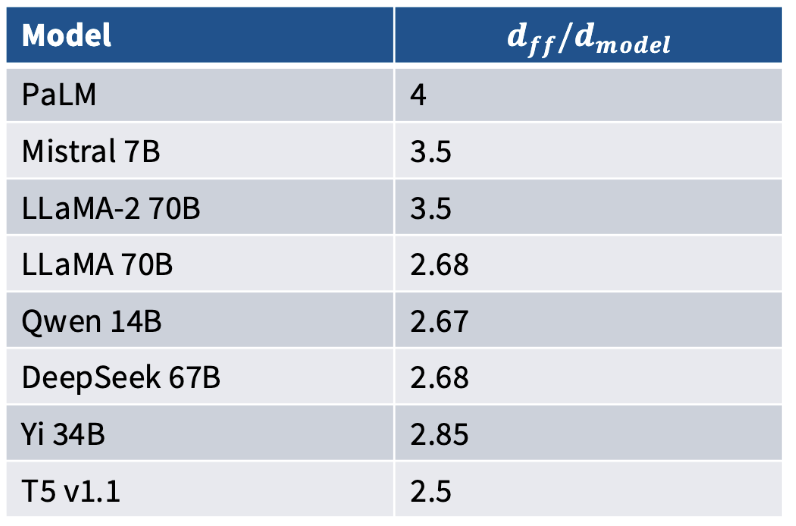
\includegraphics[width=0.65\linewidth]{figs/lec3/lec3.20.png}
  \captionof{figure}{Examples of GLU Dimensions}
\end{figure}

Models are roughly in this range, though PaLM, LLaMA2 and Mistral are slightly larger.

\subsubsection{Exception 2 - T5}~{}

绝大部分LLM的参数都比较相似,除了T5,它有着很大胆的设置。

在他们的11B模型中,他们设置:
\begin{align*}
  d_{ff} &= 65536\\
  d_{model} &= 1024
\end{align*}

\begin{figure}[htbp]
  \centering
  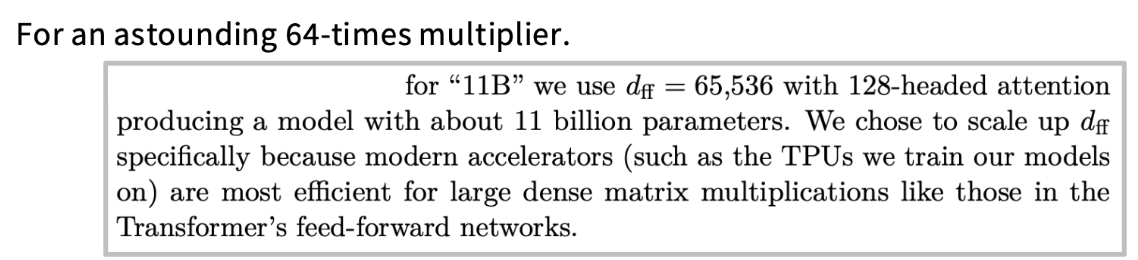
\includegraphics[width=0.8\linewidth]{figs/lec3/lec3.21.png}
  \captionof{figure}{Reason for the 64-multipliers in T-5 Model}
\end{figure}

\begin{figure}[htbp]
  \centering
  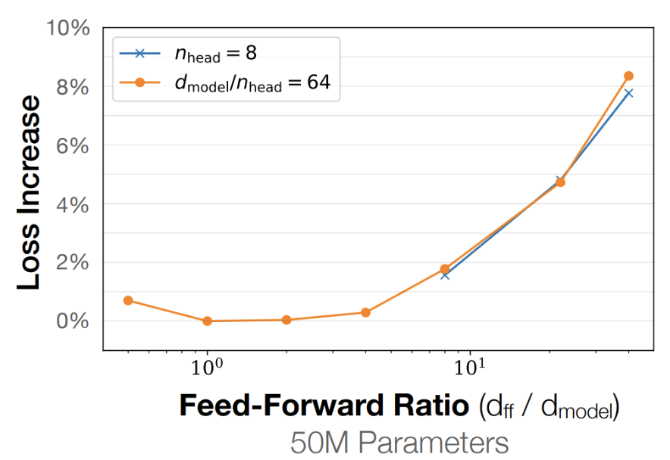
\includegraphics[width=0.8\linewidth]{figs/lec3/lec3.22.png}
  \captionof{figure}{The range of the ratio}
\end{figure}

\textbf{这个比例通常在4左右}


\clearpage
\subsection{Head Dimension, Heads number and Model Dimension}

在多头注意力机制(Multi-Head Attention, MHA)中,有三个核心维度:  

\begin{itemize}
    \item \textbf{模型维度} $d_{\text{model}}$:整个 embedding 的维度,输入与输出向量的维度均为 $d_{\text{model}}$。
    \item \textbf{头维度} $d_{\text{head}}$:单个注意力头所使用的子空间维度。
    \item \textbf{头的数量} $h$:并行的注意力头个数。
\end{itemize}

三者之间存在如下基本约束关系:
\[
    d_{\text{model}} = h \times d_{\text{head}}.
\]

\paragraph{计算上的直观理解.}~{}

输入序列经过线性变换后得到 $XQ \in \mathbb{R}^{n \times d_{\text{model}}}$
其中 $n$ 表示序列长度。

随后,我们将其 reshape 为
$\mathbb{R}^{n \times h \times d_{\text{head}}/h}$
再转置为$\mathbb{R}^{h \times n \times d_{\text{head}}/h}$

此时 \emph{head 维度可以类比为一个 batch 维度},从而使得不同的头能够并行计算。
由于矩阵的总大小保持不变,多头注意力在计算复杂度上与单头注意力几乎一致。

\paragraph{Head-dim 与 Model-dim 的比率.}~{}

我们可以定义一个衡量关系的比率:
\[
    \text{Ratio} = \frac{h \times d_{\text{head}}}{d_{\text{model}}}.
\]
在标准 Transformer 结构中,通常有 $\text{Ratio} = 1$。
这一经验法则保证了在参数量和计算开销不增加的情况下,实现并行化和多样化的注意力模式。



\paragraph{为何不是必须?}~{}

需要注意的是,上述关系并非严格限制。
理论上我们可以设置
\[
    d_{\text{head}} > \frac{d_{\text{model}}}{h},
\]
从而让每个头具有更强的表达能力。
不过,这样做会带来额外的计算和内存开销,因此多数模型仍然遵循 $\text{Ratio}=1$ 的实践规范。

\begin{figure}[htbp]
  \centering
  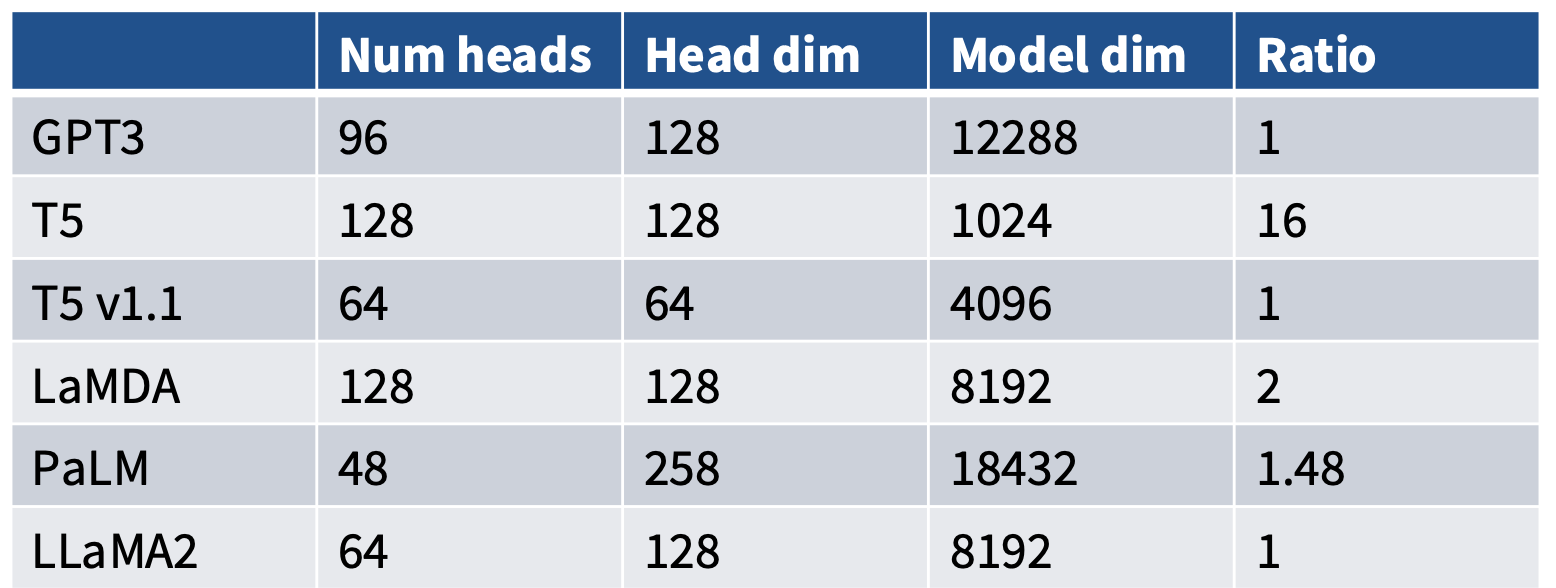
\includegraphics[width=0.8\linewidth]{figs/lec3/lec3.23.png}
  \captionof{figure}{Most models have ratios around 1.}
\end{figure}



\clearpage
\subsection{Aspect Ratio}

在 Transformer 模型设计中,\emph{aspect ratio} 通常指模型维度与网络深度的比值:
\[
    \text{Aspect Ratio} = \frac{d_{\text{model}}}{n_{\text{layer}}}.
\]

\MarginImageWithNote
  {figs/lec3/lec3.24.png}
  {\captionof{figure}{Deep models are hard to parallelize}}

\paragraph{直观理解.}
\begin{itemize}
  \item $d_{\text{model}}$ 决定了每一层的宽度,即单层的表示能力;
  \item $n_{\text{layer}}$ 决定了模型的深度,即堆叠的层数;
  \item 二者的比例刻画了模型在“宽度”和“深度”上的取舍。
\end{itemize}

\Remark{
\textbf{  Extremely deep models are harder to parallelize and have higher latency.
}}

在增加深度(scaling depth)时会遇到限制。因为深度意味着层与层之间存在严格的顺序依赖,每一层的计算必须等待上一层完成。
这导致深度扩展无法跨机器或设备进行并行化。相比之下,增加宽度(scaling width)更容易并行化,可以在成千上万台设备上同时分布计算。因此,在计算资源受限的情况下,深度扩展有一定限制。


\begin{figure}[htbp]
  \centering
  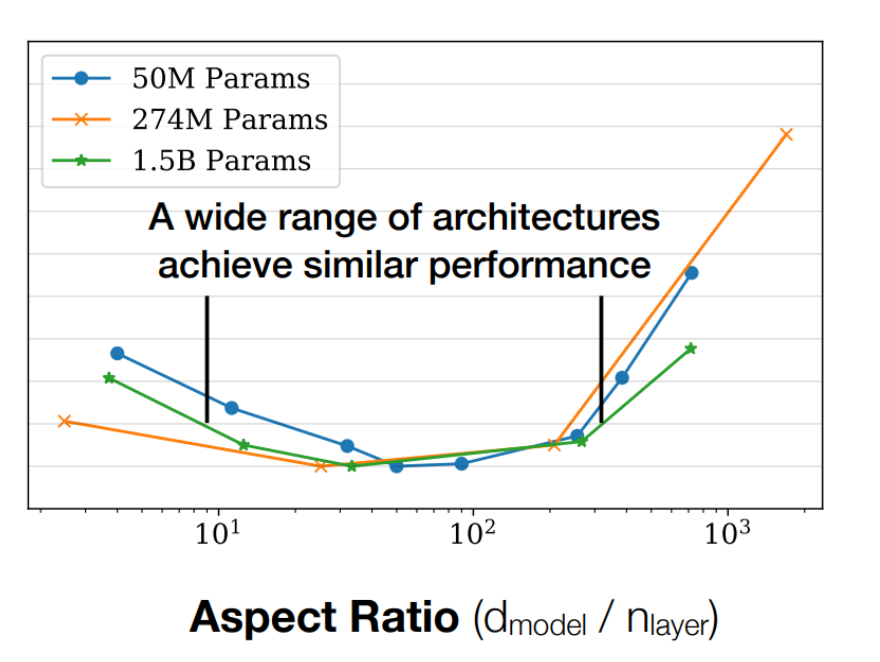
\includegraphics[width=0.8\linewidth]{figs/lec3/lec3.25.png}
  \captionof{figure}{Loss Increase vs. Aspect Ratio$(d_{model}/n_{layer})$}
\end{figure}

\clearpage
\subsection{Vocabulary Size}

\begin{figure}[htbp]
  \centering
  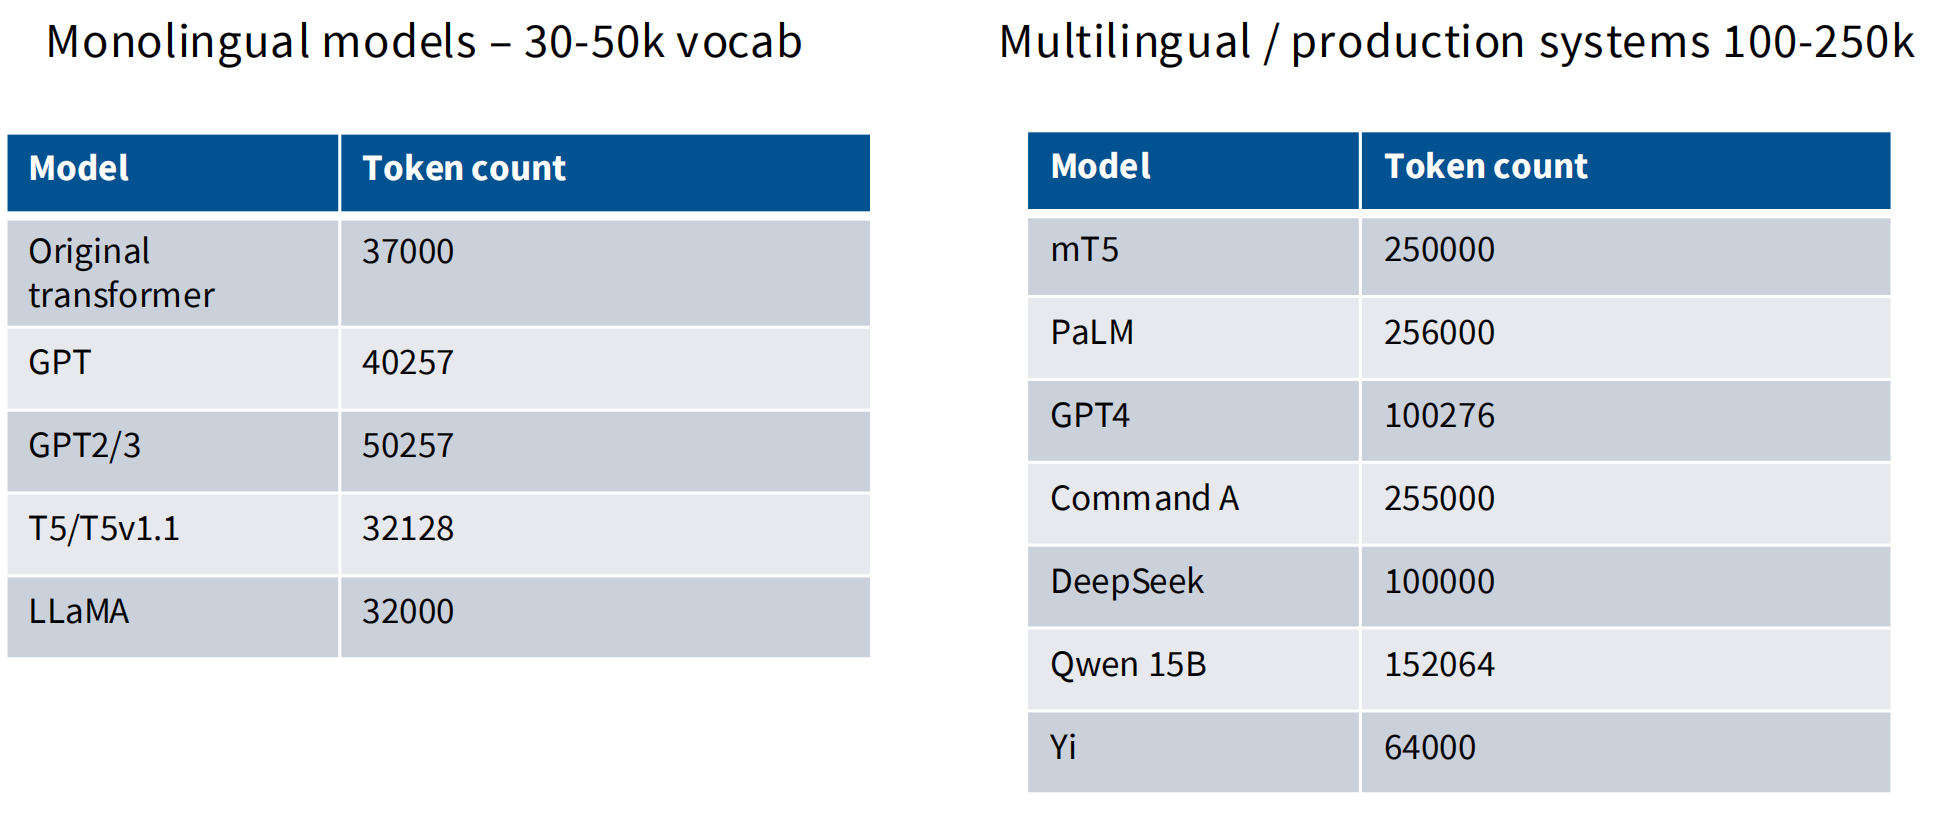
\includegraphics[width=0.8\linewidth]{figs/lec3/lec3.26.png}
  \captionof{figure}{Vocabulary Examples}
\end{figure}

Monolingual vocabs don't need to be huge, but multilingual ones do.

\subsection{Regularization}

\QA{Do we need regularization during pretraining?}
{
\textbf{Arguments against:}
\begin{itemize}
  \item There is \textit{a lot} of data (trillions of tokens), more than parameters.
  \item SGD only does a single pass on a corpus(hard to memorize)
\end{itemize}
}

\MarginNote{
\Definition{Pretraining}{
Pre-training is the initial phase of training an LLM where it learns from a large, diverse dataset of often trillions of tokens. The goal here is to develop a broad understanding of language, context, and various types of knowledge. Pre-training is usually MASSIVELY computationally expensive and requires HUGE amounts of data. We're often talking in the millions of dollars when pre-training models. This is one of the primary reasons I am personally skeptical of the idea of open source overtaking commercial models, since most open-weight LLMs still had to come from a corporation making the initial investment in pre-training. Suffice it to say as a beginner, you will not be doing any pre-training.
}

\Definition{Fine-tuning}{
Fine-tuning is where you take an already-pre-trained model and further train it on a more specific dataset. This dataset is typically smaller and focused on a particular domain or task. The purpose of fine-tuning is to adapt the model to perform better in specific scenarios or on tasks that were not well covered during pre-training. The new knowledge added during fine-tuning is more about enhancing the model's performance in specific contexts rather than broadly expanding its general knowledge.
}
}



\paragraph{Dropout and weigty decay in practice}~{}

\Definition{Dropout}{
\emph{Dropout} 是一种常见的正则化方法,在训练过程中以概率 $p$ 随机将部分神经元的输出置零。
其核心思想是通过“随机失活”防止神经元之间的过度共适应,从而提升模型的泛化能力。
在测试阶段,所有神经元均被激活,并对输出进行缩放,以保证期望一致。
}

\Definition{Weight Decay}{
\emph{Weight Decay} 是通过在损失函数中加入参数范数惩罚项来实现的正则化方法。
最常见的形式是 $L_2$ 正则化:
\[
    L_{\text{reg}} = L_{\text{original}} + \lambda \|\theta\|_2^2,
\]
其中 $\theta$ 为模型参数,$\lambda$ 为权重衰减系数。
这种方法通过抑制参数过大,间接限制了模型容量,降低过拟合风险。
}
\clearpage

\MarginImageWithNote
  {figs/lec3/lec3.27.png}
  {\captionof{figure}{Dropout and weight decay Examples}}

\textbf{Many older models used dropout during pretraining.\\
Newer models (except Qwen) rely only on weight decay.
}
\begin{figure}[htbp]
  \centering
  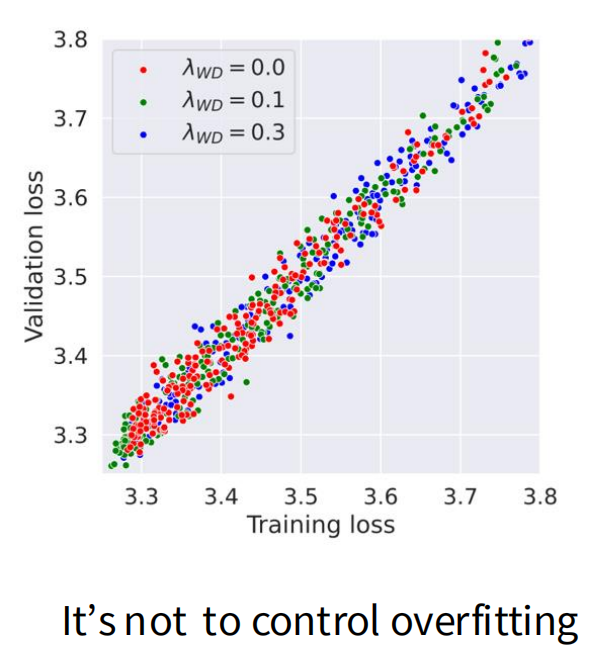
\includegraphics[width=0.5\linewidth]{figs/lec3/lec3.28.png}
  \captionof{figure}{权重衰减(Weight Decay)在大规模预训练中并不是用来防止过拟合的。
如图所示,不同的 $\lambda_{WD}$ 对训练损失与验证损失的差距几乎没有影响,
说明其主要作用并非控制过拟合,而是影响优化动态。}
\end{figure}

\begin{figure}[htbp]
  \centering
  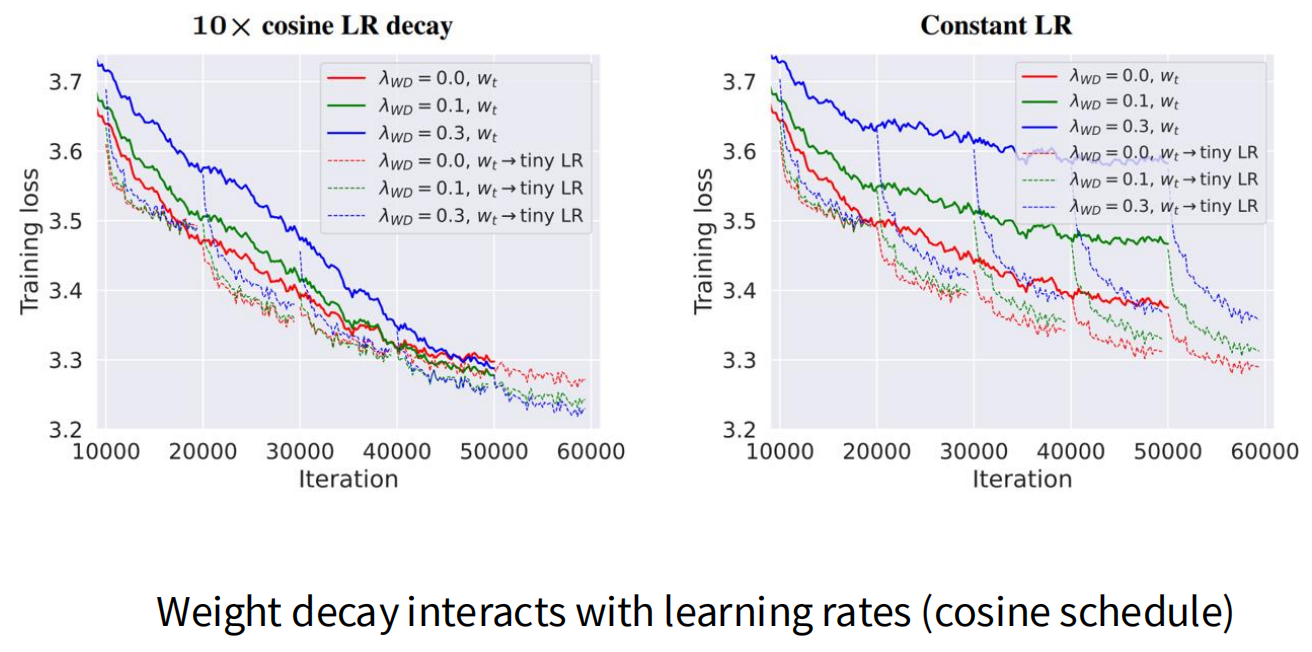
\includegraphics[width=0.7\linewidth]{figs/lec3/lec3.29.png}
  \captionof{figure}{\textbf{Weight decay interacts with learning rates(cosine schedule)}
在余弦退火 (cosine LR decay, 左) 和常数学习率 (constant LR, 右) 下,
不同 $\lambda_{WD}$ 导致了明显不同的收敛轨迹。
这表明 Weight Decay 更像是一种优化调节器,而非单纯的正则化手段。}
\end{figure}




\clearpage
{\chaptoc\noindent\begin{minipage}[inner sep=0,outer sep=0]{0.9\linewidth}\section{Stability tricks}\end{minipage}}
\\
\textbf{Recently, lots of attention on stable training.}


\begin{figure}[htbp]
  \centering
  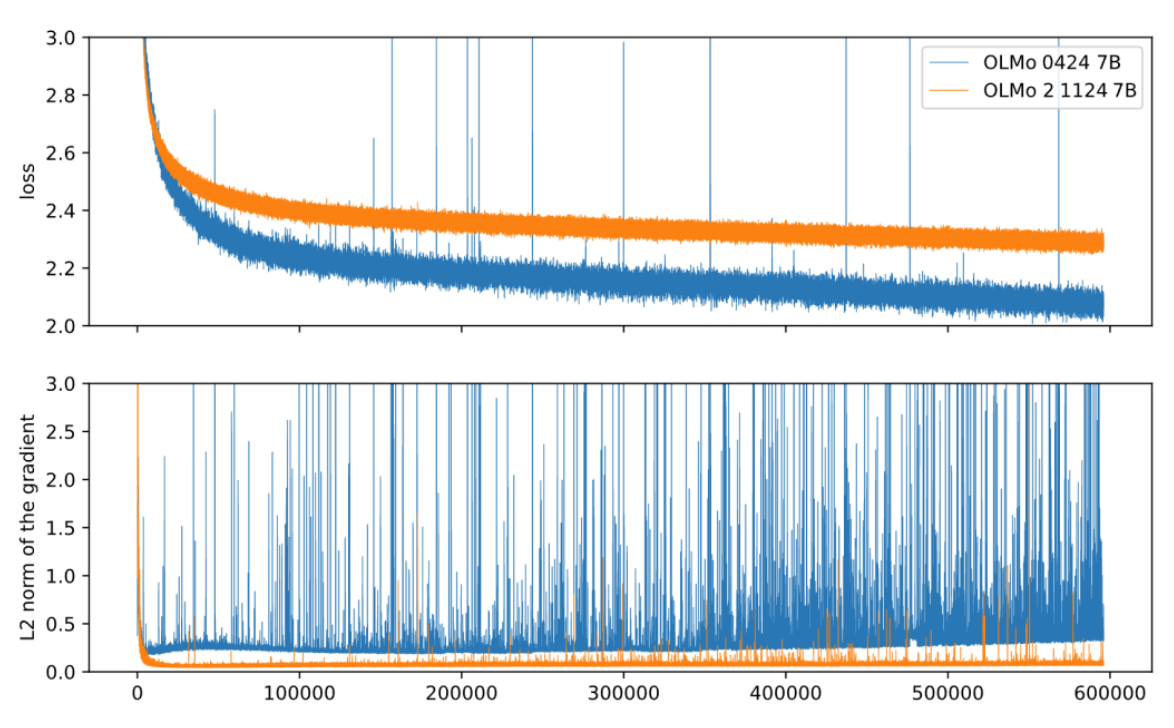
\includegraphics[width=0.7\linewidth]{figs/lec3/lec3.30.png}
  \captionof{figure}{训练过程中 loss vs. L2 Gradient}
\end{figure}

上图展示了 OLMo 0424 7B 与 OLMo 2 1124 7B 的训练损失曲线,
可以看到 OLMo 0424 在相同迭代下达到更低的 loss。
下图展示了对应的梯度 $L_2$ 范数,
其中 OLMo 0424 的梯度波动显著更大,
而 OLMo 2 1124 的梯度曲线更加平滑,
表明两者在优化稳定性上的显著差异。

\subsection{Output Softmax Stability}

\QA{Why these spikes happen?}
{\textbf{Be aware of Softmax! }}

\paragraph{原因分析.}
\begin{itemize}
    \item \textbf{指数爆炸 (Overflow).}  \\
    Softmax 会将 logits 通过指数映射:
    \[
        p_i = \frac{\exp(z_i)}{\sum_j \exp(z_j)}.
    \]
    当某个 $z_i$ 的绝对值过大时(尤其是正数),指数函数会导致数值溢出,
    使概率分布极度偏斜,从而放大梯度,造成 loss 的尖峰。
    
    \item \textbf{分母过小 (Underflow / Division by tiny number).}  \\
    若所有 $z_j$ 都非常负,$\sum_j \exp(z_j)$ 会接近零,
    这相当于在 softmax 中出现了近似“除零”操作,
    使得 $p_i$ 的数值不稳定,进一步导致交叉熵 loss$-\log(p_{y})$ 变得极大,从而出现训练曲线的 spike。
    
    \item \textbf{梯度放大.}  \\
    在反向传播中,softmax 的梯度为 $\nabla_z = p - y$。
    当 $p$ 接近 $0$ 或 $1$ 时,梯度可能出现剧烈波动,
    放大了上述数值不稳定性带来的影响。
\end{itemize}

\clearpage
\paragraph{缓解方法.}~{}

\subparagraph{Softmax 定义.}
给定输入 $x$,模型会为词表中的每个候选 $r \in \{1, \dots, |V|\}$ 产生一个未归一化分数(logit) $U_r(x)$。  
Softmax 将这些 logits 转换为概率分布:
\[
    P(r \mid x) = \frac{\exp\big(U_r(x)\big)}{\sum_{r'=1}^{|V|} \exp\big(U_{r'}(x)\big)}.
\]
其中:
\begin{itemize}
    \item $U_r(x)$:输入 $x$ 对应类别 $r$ 的 logit,通常由线性层或仿射变换得到;
    \item $|V|$:词表大小;
    \item $Z(x) = \sum_{r'=1}^{|V|} \exp(U_{r'}(x))$:归一化因子 (partition function)。
\end{itemize}

\subparagraph{取对数.}
语言建模通常最大化对数似然:
\[
    \log P(r \mid x) = \log \frac{\exp(U_r(x))}{Z(x)}.
\]
拆解为:
\[
    \log P(r \mid x) = U_r(x) - \log Z(x).
\]

\subparagraph{原始损失函数.}
在整个训练数据集 $\{x_i\}$ 上,损失函数为:
\[
    L_{\text{orig}} = \sum_i \log P(x_i).
\]

\subparagraph{加入正则项.}
为了缓解数值不稳定 (spikes),可对分母 $Z(x)$ 施加惩罚,鼓励其保持在合理范围:
\[
    L = \sum_i \Big[ \log P(x_i) - \alpha \big(\log Z(x_i)\big)^2 \Big],
\]
其中 $\alpha$ 为正则化系数。该正则项等价于鼓励 $logZ(x) \approx 0 \rightarrow Z(x) \approx 1$,从而避免溢出或近似除零。

\subparagraph{推导流程图.}
\begin{center}
\begin{tikzpicture}[node distance=2cm, auto, >=stealth, thick]
    \tikzstyle{box} = [rectangle, draw=black, rounded corners, minimum height=1cm, minimum width=3.5cm, align=center]

    % Nodes
    \node[box] (softmax) {Softmax 定义 \\ $P(r|x) = \frac{e^{U_r(x)}}{\sum_{r'} e^{U_{r'}(x)}}$};
    \node[box, below of=softmax] (log) {取对数 \\ $\log P(r|x) = U_r(x) - \log Z(x)$};
    \node[box, below of=log] (loss) {原始损失函数 \\ $L_{\text{orig}} = \sum_i \log P(x_i)$};
    \node[box, below of=loss] (reg) {加入正则项 \\ $L = \sum_i [\log P(x_i) - \alpha (\log Z(x_i))^2]$};

    % Arrows
    \draw[->] (softmax) -- (log);
    \draw[->] (log) -- (loss);
    \draw[->] (loss) -- (reg);
\end{tikzpicture}
\end{center}

\clearpage
\subsection{Attention Softmax Stability - the QK norm}

\paragraph{\textbf{Motivation}}~{}

在 Transformer 自注意力机制中,注意力权重计算依赖于以下公式:
\[
\mathrm{Attention}(Q,K,V) = \mathrm{Softmax}\!\left(\frac{QK^\top}{\sqrt{d_k}}\right) V,
\]
其中 $Q, K \in \mathbb{R}^{n \times d_k}$ 是 query 和 key,$d_k$ 是 head 的维度,通常用于缩放 dot-product。

The key issue of the standard dot-product attention is that: the values going into softmax can get super large, which ends up making the attention too sharp or too “winner-take-all” like below:

\Example{Problem of standard dot-product}
{
\begin{align*}
&\text{softmax}([760, 752, 750])\\
&= \text{softmax}([12, 4, 2])\\
&=[0.99962, 0.00034, 0.00005]
\end{align*}  

Where both the 760 and 12 take most \textbf{“attention”}. That can actually hurt learning, especially when we want the model to spread its attention around a bit more. Also, the softmax only cares about the differences between values instead of their magnitudes.

}

\paragraph{Query-Key Normalization(QK-Norm)}~{}

Instead of using raw dot products between queries and keys, they normalize both vectors using L2 norm (so now we're working with cosine similarity).

\[
\text{cosine\_similarity}\!\big(\vec{a}, \vec{b}\big) 
= \frac{\vec{a} \cdot \vec{b}}{\|\vec{a}\|_2 \, \|\vec{b}\|_2}.
\]

However, the scale in the softmax still somehow matters since the range of cosine similarity is $[-1, 1]$. 
\textbf{The expressive ability may be insufficient when cosine similarity is combined with Softmax. }


Therefore, \textbf{adding a learnable temperature parameter} or something similar is important. The specific operation of the \textbf{QK Norm} is to 
\begin{itemize}
  \item first normalize $Q$ and $K$
  \item then multiply them with a \textbf{learnable scalar weight}.
\end{itemize}  

That way, the values going into softmax stay in a more useful range: not too big, not too small.
\paragraph{With QK-Norm}~{}

The attention weights are computed as
\[
    \mathrm{Attention}(Q,K,V) 
    = \mathrm{Softmax} \big( g * \hat Q \hat K^\top \big) V,
\]
where $g$ is a learnable scale factor (temperature).  
Here, $\hat Q$ and $\hat K$ denote $Q$ and $K$ after $\ell_2$-normalization applied along their head dimensions.  
Because the vector norms are normalized, the denominator $\sqrt{d_k}$ in the standard formulation can be omitted.

\begin{figure}[htbp]
  \centering
  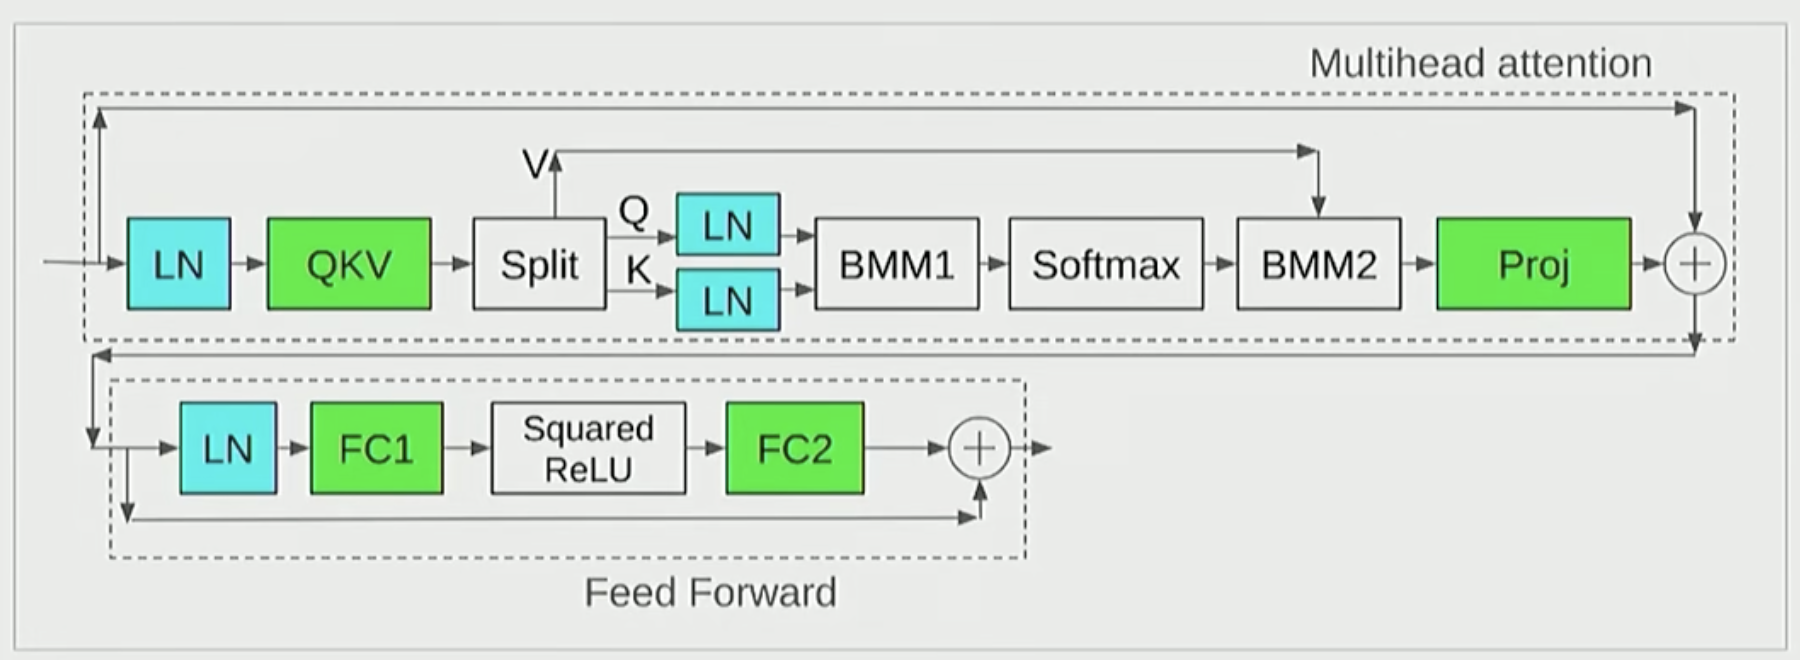
\includegraphics[width=0.7\linewidth]{figs/lec3/lec3.31.png}
  \captionof{figure}{Transformer Architecture with QK norm}
\end{figure}

\paragraph{Difference with Usual Normalization.}~{}

It is important to distinguish QK-Norm from standard normalization methods such as Batch Normalization or Layer Normalization.  
These common techniques perform \emph{standardization}, i.e.,
\[
    \hat x = \frac{x - \mu}{\sigma},
\]
which enforces zero mean and unit variance across a batch or feature dimension, but does not constrain the vector length.  \\
In contrast, QK-Norm applies true $\ell_2$ normalization:
\[
    \hat q = \frac{q}{\|q\|_2}, \qquad \hat k = \frac{k}{\|k\|_2},
\]
ensuring each query and key vector has unit norm.  \\
Thus, the dot product between $\hat q$ and $\hat k$ becomes a cosine similarity, strictly bounded in $[-1,1]$.  \\
This makes QK-Norm fundamentally different from standard normalization: it directly controls vector magnitude rather than just its statistical distribution.



\subsection{Logit Soft-Capping}

在注意力机制中,logits 来自 $QK^\top$(或其变体)。若 logits 过大,Softmax 会趋向 one-hot,
导致梯度爆炸或训练不稳定。为缓解这一问题,可以对 logits 进行 \emph{soft-capping},
即通过一个光滑的函数将其压缩到合理的范围,而不是采用硬截断。


\Definition{Logit Soft-Capping}{
We cap logits in each attention layer as well as in the final layer, 
so that the values remain bounded within $[-\text{soft\_cap}, +\text{soft\_cap}]$.  
More specifically, we cap the logits with the following function: \\
Given raw logits $z$, the capping is applied as:
\[
    z \;\leftarrow\; \text{soft\_cap} \cdot \tanh\!\left(\frac{z}{\text{soft\_cap}}\right).
\]
We set the soft-cap parameter to 50.0 for the self-attention layers and to 30.0 for the final layer.
}



\subparagraph{Effect on Attention.}~{}

在 softmax 之前应用 soft-capping:
\[
    \mathrm{Attention}(Q,K,V) = \mathrm{Softmax}(z')V,
\]
使得 logits 不会无限增大,从而避免了 softmax 输出塌陷为 one-hot 分布,提升训练稳定性。

\subparagraph{Comparison with QK-Norm.}
\begin{itemize}
    \item QK-Norm 控制的是输入向量 $Q, K$ 的范数,从源头抑制 logits 爆炸;
    \item Soft-capping 则直接作用在 logits 上,通过平滑函数限制其幅值;
    \item 两者可以结合使用(称为 \emph{QK-Norm + SoftCap}),进一步提升稳定性。
\end{itemize}




\clearpage
{\chaptoc\noindent\begin{minipage}[inner sep=0,outer sep=0]{0.9\linewidth}\section{Attention Heads}\end{minipage}}
\\

\subsection{Grouped-Query Attention \& Multi-Query Attention}


\paragraph{Motivation.}~{}

In standard multi-head attention, each head has its own set of $Q, K, V$ projections.
This design is \textbf{expressive} but \textbf{computationally expensive}, 
as storing and computing with all keys and values becomes costly when scaling to large models.

Let's think about the compute involved for attention:


\begin{figure}[htbp]
  \centering
  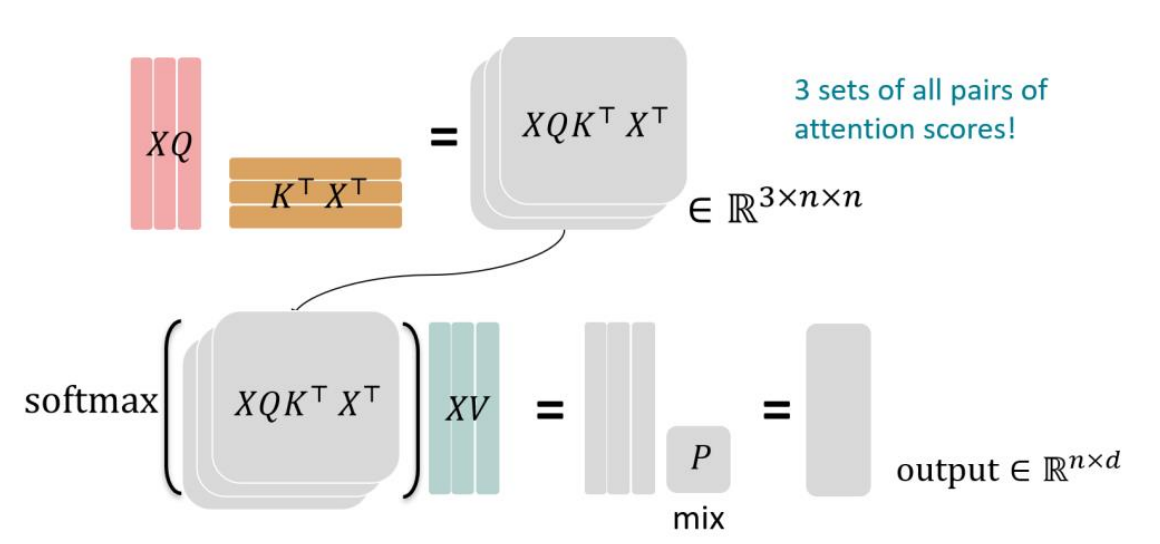
\includegraphics[width=0.7\linewidth]{figs/lec3/lec3.32.png}
  \captionof{figure}{Computation in attention}
\end{figure}

\Remark{
  \textbf{Total arithmetric operations $(bnd^2)$, total memory accesses($bnd + bhn^2 + d^2$)}
}

\paragraph{Arithmetic Intensity.}~{}

\Definition{Arithmetic Intensity}{
Arithmetic Intensity (AI) 指的是 \emph{每次内存访问所能完成的算术运算量},反映了计算与内存访问之间的平衡关系。  

\[
  \text{AI} = \frac{\text{\# arithmetic ops}}{\text{\# memory accesses}}
\]

在矩阵乘法等注意力计算中,AI 的数量级近似为:
\[
  \text{AI} \;\sim\; \Big(\tfrac{1}{k} + \tfrac{1}{bn}\Big)^{-1},
\]
其中 $k$ 为 head 维度,$b$ 为 batch size,$n$ 为序列长度。  
这意味着当 $b$ 与 $n$ 较大时,AI 值也随之提高,能够充分利用 GPU 的算力资源。
}

\clearpage
\MarginNote{
\textbf{Matrix Multiplication Complexity.} \\
Multiplying an $m \times k$ matrix with a $k \times n$ matrix requires
\[
\mathcal{O}(mkn)
\]
arithmetic operations (dot products of rows and columns). \\
\medskip
\emph{Example:} In attention, $Q \in \mathbb{R}^{n \times d}$ and $K^\top \in \mathbb{R}^{d \times n}$, 
so the complexity is $\mathcal{O}(n \cdot d \cdot n) = \mathcal{O}(nd^2)$ (per batch). \\
\medskip
This forms the dominant term in the cost of computing $QK^\top$.
}


\Proposition{Complexity of Multi-Head Attention}{
Consider a batch of \textit{$b$} sequences, each of length \textit{$n$}, with model dimension \textit{$d$} and \textit{$h$} attention heads.  \\
The total complexity of multi-head attention can be decomposed into arithmetic operations and memory accesses.

\subparagraph{Arithmetic Operations.}
The dominant cost arises from computing the attention scores:
\[
    \text{Attention}(Q,K,V) = \mathrm{Softmax}(QK^\top)V.
\]
Here,
\[
    Q \in \mathbb{R}^{b \times n \times d}, 
    \quad K \in \mathbb{R}^{b \times n \times d}.
\]
The matrix multiplication $QK^\top$ has complexity
\[
    \mathcal{O}(b \cdot n \cdot d^2) = \mathcal{O}(bnd^2).
\]

Thus,
\[
    \text{Total Arithmetic Operations} = bnd^2.
\]

\subparagraph{Memory Accesses.}
The memory cost consists of three parts:
\begin{itemize}
    \item \textbf{Input projections:} loading $X \in \mathbb{R}^{b \times n \times d}$ to compute $Q,K,V$, costing $bnd$ accesses.
    \item \textbf{Attention scores:} for each head, storing $QK^\top \in \mathbb{R}^{n \times n}$, repeated across $h$ heads, giving $bhn^2$ accesses.
    \item \textbf{Output projection:} the output is mapped back to $\mathbb{R}^{d}$ via $W^O \in \mathbb{R}^{hd \times d}$, requiring $d^2$ accesses.
\end{itemize}
Summing these,
\[
    \text{Total Memory Accesses} = bnd + bhn^2 + d^2.
\]

\subparagraph{Conclusion.}
The computational and memory complexity of multi-head attention are:
\[
    \text{Arithmetic Ops} = bnd^2, \qquad
    \text{Memory Accesses} = bnd + bhn^2 + d^2.
\]
}

\QA{What about the \textit{incremental case} when we generate text?}
{
\\
\textbf{Key difference:} During autoregressive generation, the model cannot parallelize the computation across all tokens.\\
Instead, tokens must be generated \emph{step by step}, each conditioned on the previously generated context.

\subparagraph{Challenge.}~{}

Naively re-computing attention at every step would require re-processing all past tokens,
leading to a quadratic time cost across the entire generation process.

\subparagraph{Solution: KV Cache.}~{}

To avoid redundant computation, we maintain a \emph{key-value (KV) cache}:
{\color{tred}
\begin{itemize}
    \item At each generation step, newly computed $K,V$ vectors are appended to the cache.
    \item The current query $Q_t$ only attends to cached $(K,V)$ pairs from all past steps.
    \item This transforms the per-step cost from $\mathcal{O}(t^2)$ re-computation into $\mathcal{O}(t)$ incremental updates.
\end{itemize}
}

\subparagraph{Summary.}~{}

In incremental generation, the key difference is the loss of full parallelism.\\
The KV cache is the practical mechanism that enables efficient autoregressive decoding by
reusing past $K,V$ representations rather than recomputing them.
}


\begin{figure}[htbp]
  \centering
  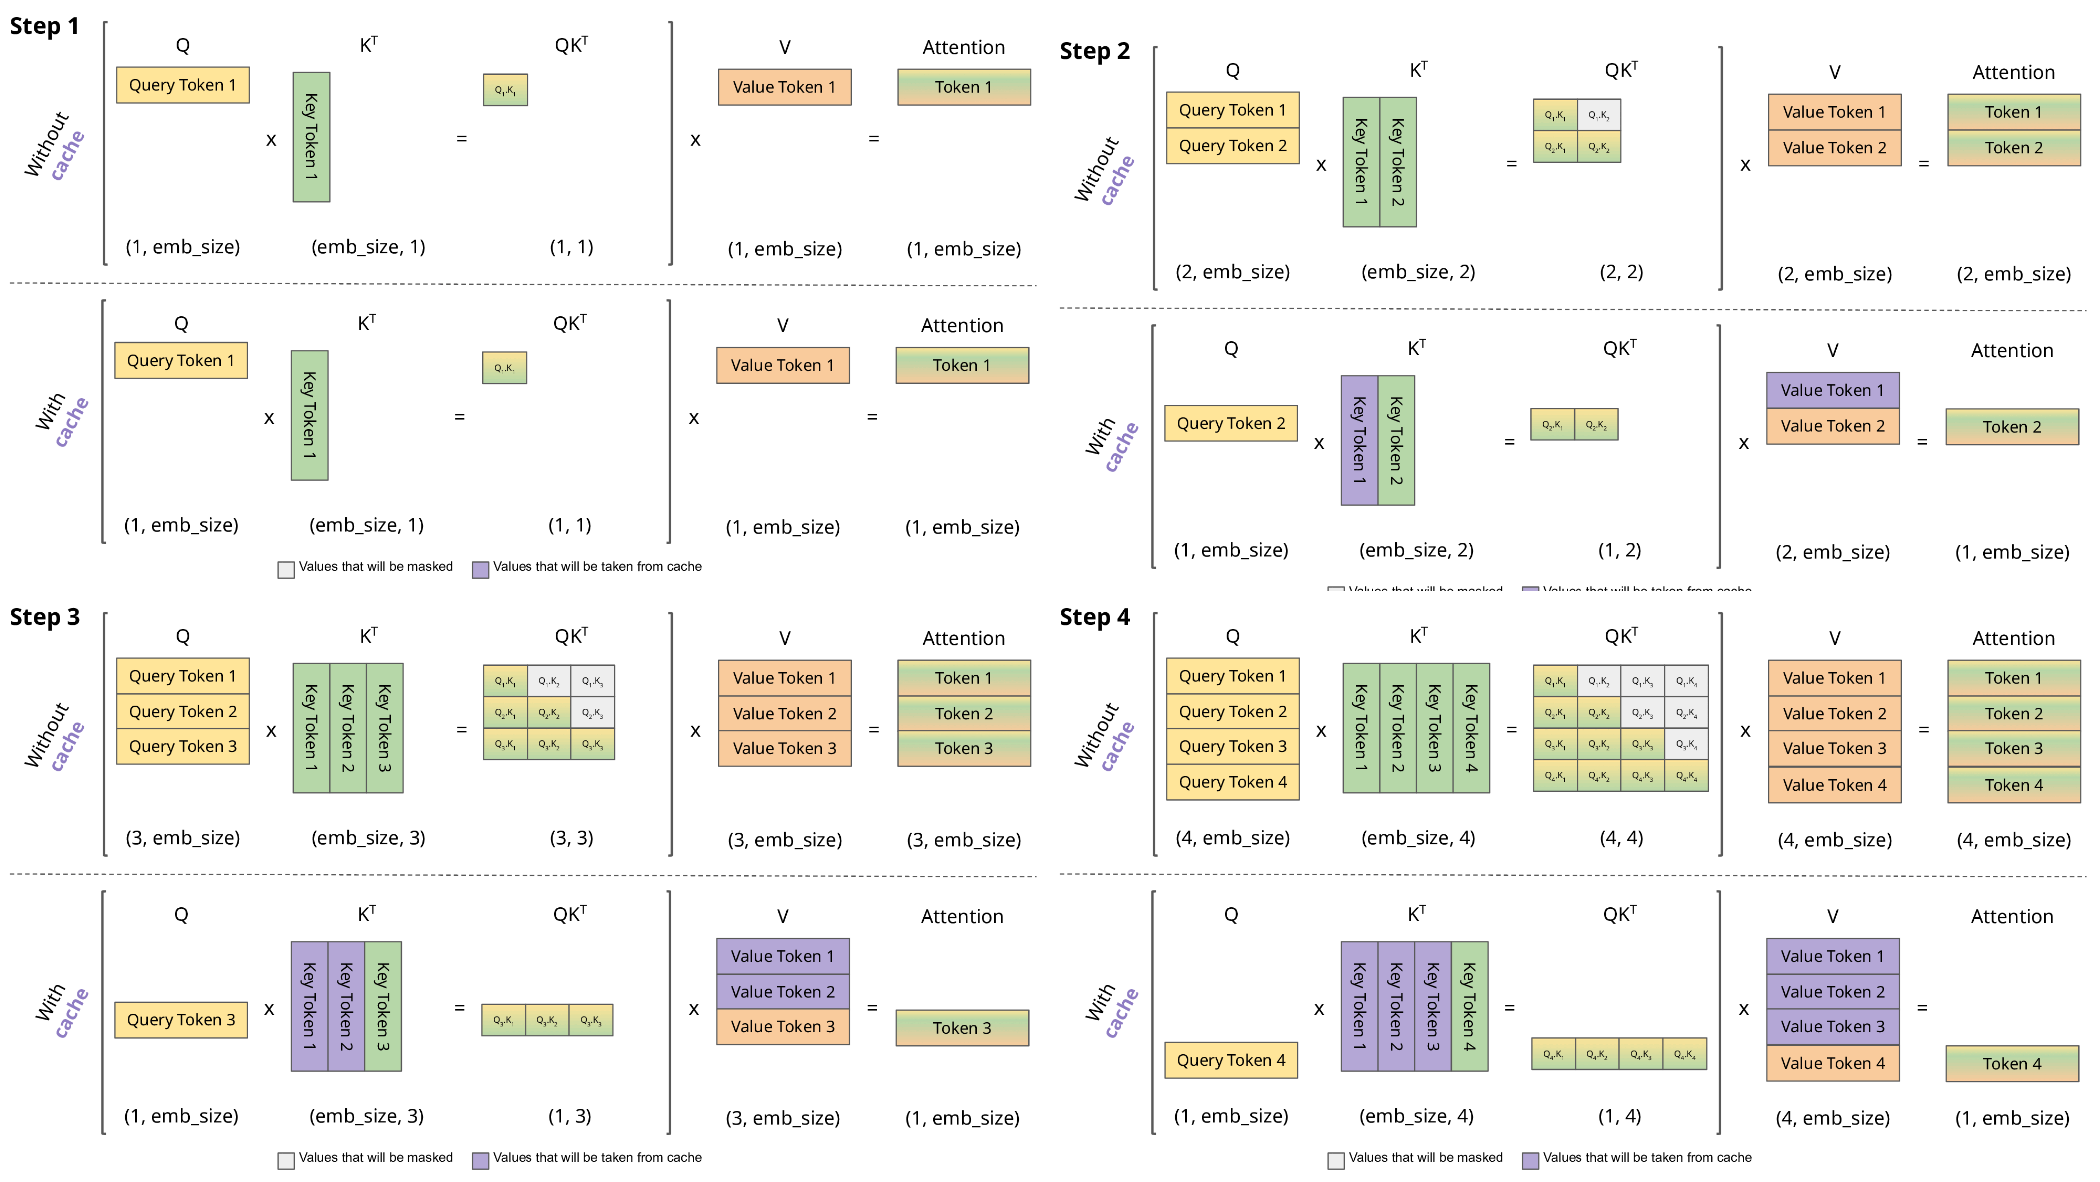
\includegraphics[width=1\linewidth]{figs/lec3/lec3.33.png}
  \captionof{figure}{KV Cache示意图,上一排是without KV cache, 下一排是with KV Cache.}
\end{figure}

\clearpage
\QA{What's the incremental arithmetic intensity?}
{{\color{dblue} The core idea: With KV cache, Ks and Vs are generated incrementally as each token.}\\

The system only multiply the absolute necessary keys and values, since all of the intermediate computations are saved. There is no waste of any matrix or vector multiplies.\\

\[
\text{Arithmetic ops:} \quad b n d^{2}
\]

\[
\text{Memory accesses:} \quad b n^{2} d \;+\; n d^{2}
\]


其中:
- $b n^{2} d$: 读写/生成整张 $n \times n$ 的注意力相关数据(随序列长平方增长,且每项含 $d$)。\\
- $n d^{2}$: QKV 与输出投影的读写(与模型维度平方相关)。

\[
\Rightarrow \quad 
AI_{\text{base}}
= \frac{b n d^{2}}{b n^{2} d + n d^{2}}
= \Theta \!\left( \left( \tfrac{n}{d} + \tfrac{1}{b} \right)^{-1} \right)
\]
need large batches + short seq length(n) or big model dimension (d)

\textbf{这其实不符合我们的期望}
}

\paragraph{MQA(Multi-Query Attention)}~{}

\textbf{{\color{tred} Key idea – have multiple queries, but just one dimension for keys and values.
That will have much fewer items to move in and out of memory(KV Cache.)}
}

\begin{figure}[htbp]
  \centering
  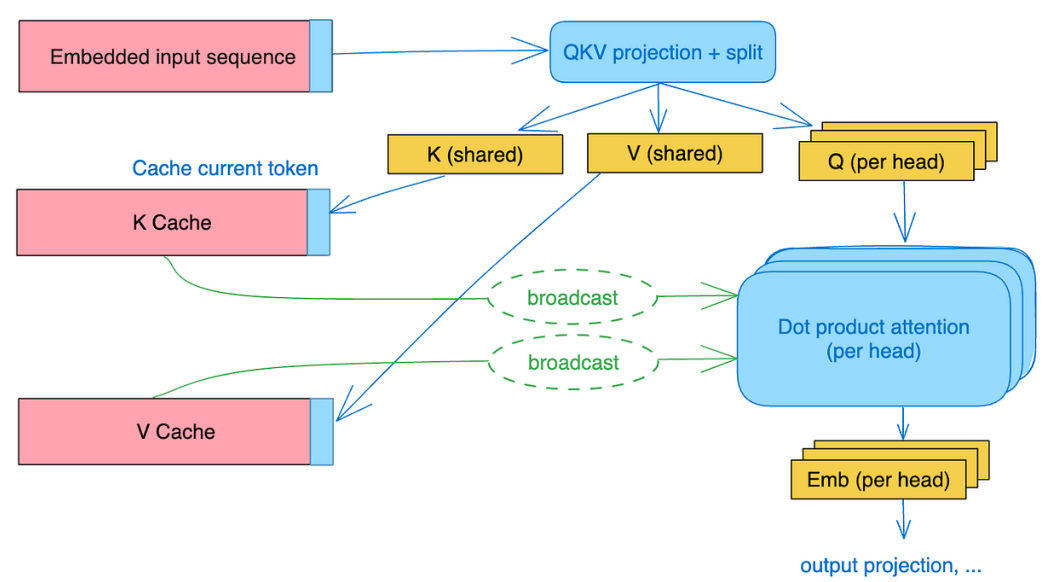
\includegraphics[width=1\linewidth]{figs/lec3/lec3.34.png}
  \captionof{figure}{MQA 示意图}
\end{figure}

\subparagraph{MQA 的思想}~{}

多个 Query head 共享同一份 Key/Value。具体来说:

\begin{itemize}
  \item 每个 head 仍然有自己独立的 $Q$ 矩阵(因此表达能力保留)。
  \item 但 $K, V$ 投影矩阵只有一份(或极少数几份)。
\end{itemize}

\QA{MQA arithmetic intensity}{
\[
\text{Arithmetic ops:} \quad b n d^{2}
\]

\[
\text{Memory accesses:} \quad b n d \;+\; b n^{2} k \;+\; n d^{2}
\]

其中:$b n d$ 表示序列流动,$b n^{2} k$ 表示注意力读写($k \ll d$),$n d^{2}$ 表示投影读写。

\[
\Rightarrow \quad 
AI_{\text{MQA}}
= \frac{b n d^{2}}{b n d + b n^{2} k + n d^{2}}
= \Theta \!\left( \left( \tfrac{1}{d} + \tfrac{n}{d h} + \tfrac{1}{b} \right)^{-1} \right)
\]
}




\paragraph{GQA(Grouped-Query Attention)—按 slide 的总量}

\[
\text{Arithmetic ops:} \quad b n d^{2}
\]

\[
\text{Memory accesses:} \quad b n d \;+\; b n^{2} \tfrac{d}{g} \;+\; n d^{2}
\]

其中:
\begin{itemize}
  \item $b n d$: 序列流动过程中的必要读写。
  \item  $b n^{2} \tfrac{d}{g}$: 注意力相关数据的读写。在 GQA 中,$g$ 个 Query head 共享一份 $K/V$,等效于把 $d$ 缩小为 $d/g$。
  \item  $n d^{2}$: QKV 与输出投影的读写。
\end{itemize}
\[
\Rightarrow \quad 
AI_{\text{GQA}}
= \frac{b n d^{2}}{b n d + b n^{2} \tfrac{d}{g} + n d^{2}}
= \Theta \!\left( \left( \tfrac{1}{d} + \tfrac{n}{d \cdot g} + \tfrac{1}{b} \right)^{-1} \right)
\]


直觉:相比基线,GQA 通过 $g$ 个 head 共享 K/V 缓存,使内存访问量从 $b n^{2} d$ 降低为 $b n^{2} d/g$,因此 $AI$ 得到提升,效果介于基线与 MQA 之间。

\begin{figure}[htbp]
  \centering
  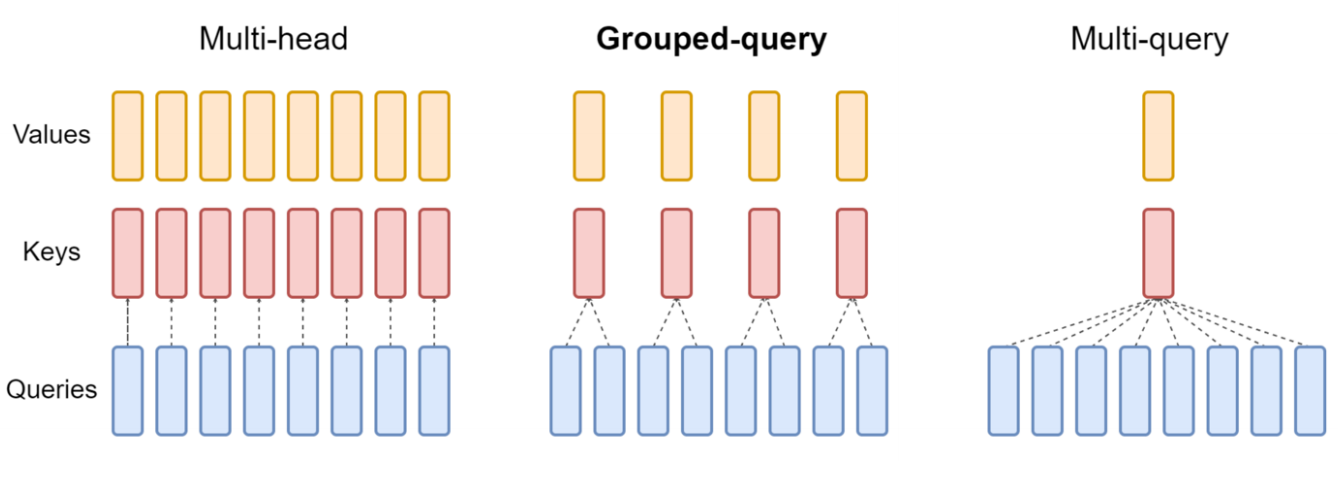
\includegraphics[width=1\linewidth]{figs/lec3/lec3.35.png}
  \captionof{figure}{GQA示意图}
\end{figure}


\clearpage
\subsection{Sparse/Sliding Window Attention}

\Definition{Sparse/Sliding Window Attention}{
传统的全局注意力计算复杂度为 $O(n^{2})$,在长序列下代价极高。  
Sparse/Sliding Window Attention 的核心思想是:  
\begin{itemize}
\item 每个 token 只与一个局部窗口(大小 $w \ll n$)中的相邻 token 进行注意力计算;  \\
\item  少量特殊位置(如段首、CLS token)可与全局交互,从而维持一定的全局建模能力。  
\end{itemize}

其复杂度下降为:
\[
\text{Arithmetic ops: } O(b n w d), 
\quad
\text{Memory: } O(b n w d + n d^{2}).
\]

优点:显著减少长序列下的算力与内存需求;  \\
缺点:丢失了完整的全局交互,需要额外机制弥补。
}

\Remark{Build sparse / structured attention that trades off expressiveness vs. runtime.}{}

\begin{figure}[htbp]
  \centering
  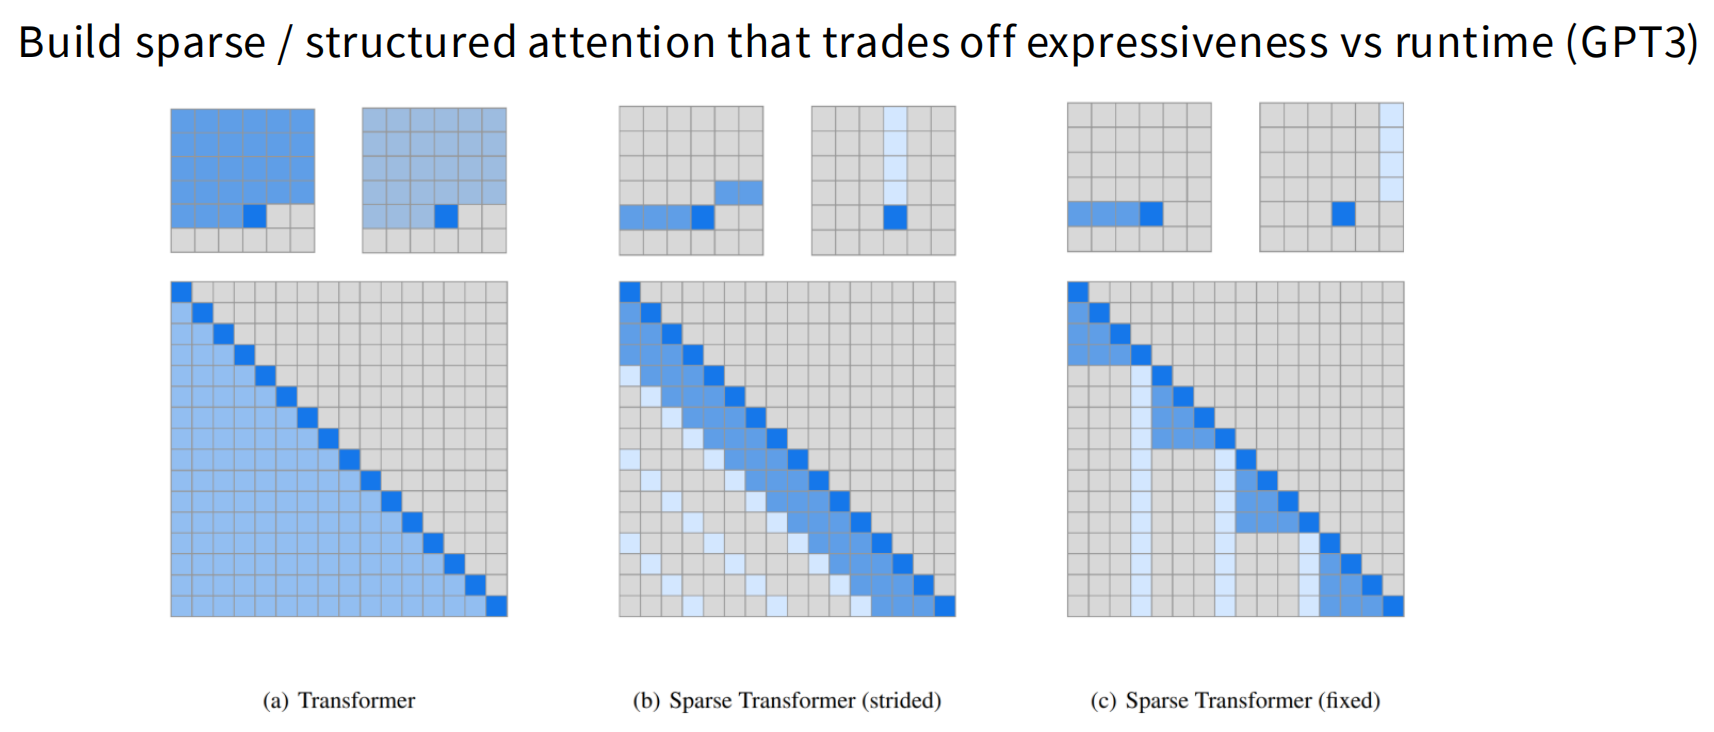
\includegraphics[width=0.8\linewidth]{figs/lec3/lec3.36.png}
  \captionof{figure}{Sparse / Sliding window attention 示意图}
\end{figure}


\begin{figure}[htbp]
  \centering
  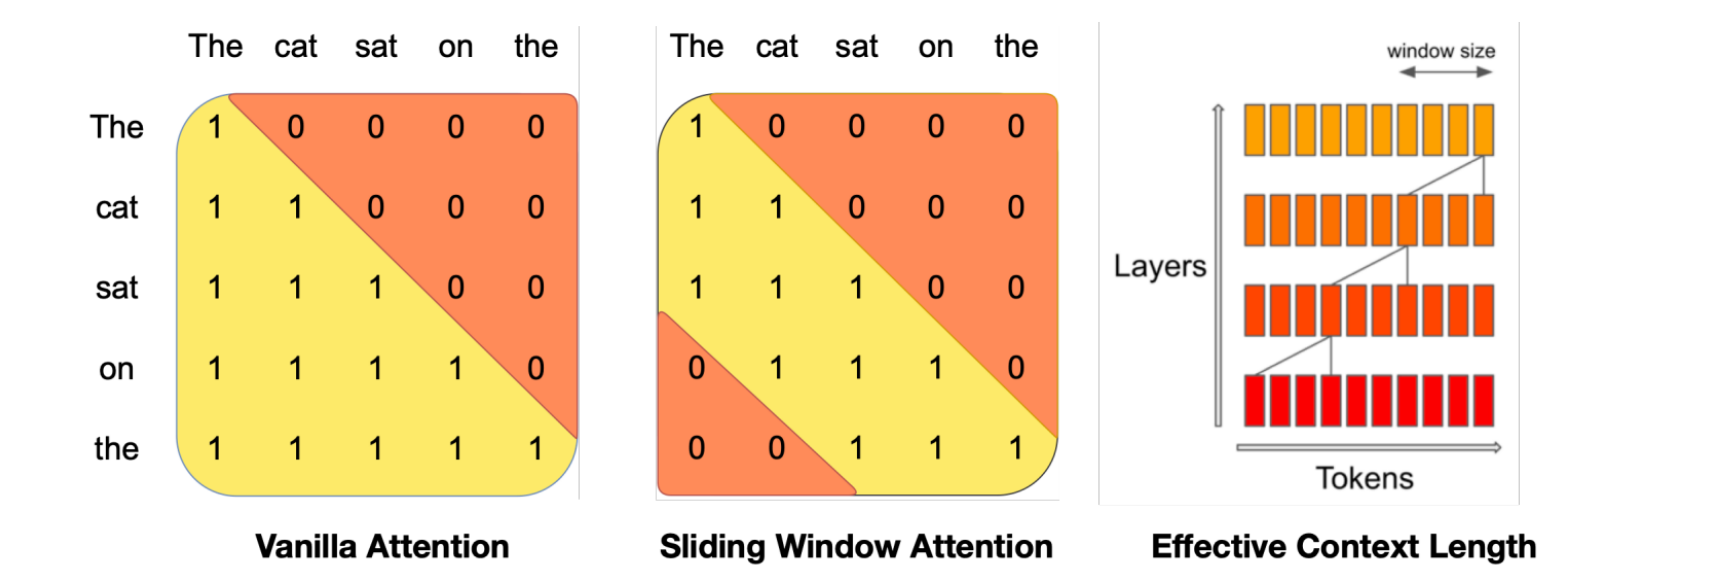
\includegraphics[width=0.8\linewidth]{figs/lec3/lec3.37.png}
  \captionof{figure}{Sliding window attention 示意图. \textbf{Just use the main part of the strided pattern.}}
\end{figure}

\clearpage
\paragraph{Current standard trick - interleave 'full' and 'LR' attention.}
\begin{figure}[htbp]
  \centering
  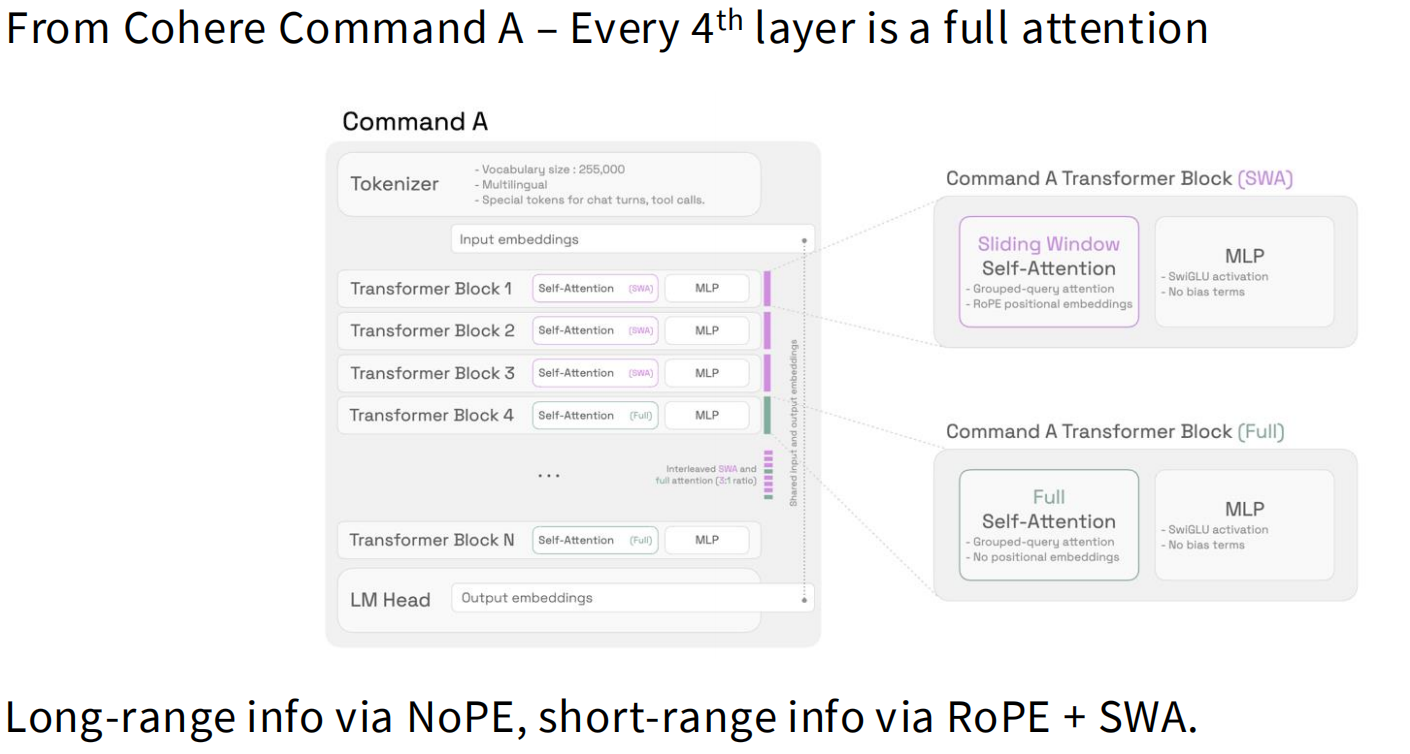
\includegraphics[width=1\linewidth]{figs/lec3/lec3.38.png}
  \captionof{figure}{Standard trick 示意图}
\end{figure}



% 图 1:OPT FLOPs 构成
% \MarginImageWithNote
%   {figs/}
%   {\captionof{figure}{}}
%   {
%   }

% \begin{figure}[htbp]
%   \centering
%   \includegraphics[width=1\linewidth]{figs/lec1/.png}
%   \caption{}
%   \label{fig:}
% \end{figure}


